\documentclass[twoside]{book}

% Packages required by doxygen
\usepackage{fixltx2e}
\usepackage{calc}
\usepackage{doxygen}
\usepackage[export]{adjustbox} % also loads graphicx
\usepackage{graphicx}
\usepackage[utf8]{inputenc}
\usepackage{makeidx}
\usepackage{multicol}
\usepackage{multirow}
\PassOptionsToPackage{warn}{textcomp}
\usepackage{textcomp}
\usepackage[nointegrals]{wasysym}
\usepackage[table]{xcolor}

% Font selection
\usepackage[T1]{fontenc}
\usepackage[scaled=.90]{helvet}
\usepackage{courier}
\usepackage{amssymb}
\usepackage{sectsty}
\renewcommand{\familydefault}{\sfdefault}
\allsectionsfont{%
  \fontseries{bc}\selectfont%
  \color{darkgray}%
}
\renewcommand{\DoxyLabelFont}{%
  \fontseries{bc}\selectfont%
  \color{darkgray}%
}
\newcommand{\+}{\discretionary{\mbox{\scriptsize$\hookleftarrow$}}{}{}}

% Page & text layout
\usepackage{geometry}
\geometry{%
  a4paper,%
  top=2.5cm,%
  bottom=2.5cm,%
  left=2.5cm,%
  right=2.5cm%
}
\tolerance=750
\hfuzz=15pt
\hbadness=750
\setlength{\emergencystretch}{15pt}
\setlength{\parindent}{0cm}
\setlength{\parskip}{3ex plus 2ex minus 2ex}
\makeatletter
\renewcommand{\paragraph}{%
  \@startsection{paragraph}{4}{0ex}{-1.0ex}{1.0ex}{%
    \normalfont\normalsize\bfseries\SS@parafont%
  }%
}
\renewcommand{\subparagraph}{%
  \@startsection{subparagraph}{5}{0ex}{-1.0ex}{1.0ex}{%
    \normalfont\normalsize\bfseries\SS@subparafont%
  }%
}
\makeatother

% Headers & footers
\usepackage{fancyhdr}
\pagestyle{fancyplain}
\fancyhead[LE]{\fancyplain{}{\bfseries\thepage}}
\fancyhead[CE]{\fancyplain{}{}}
\fancyhead[RE]{\fancyplain{}{\bfseries\leftmark}}
\fancyhead[LO]{\fancyplain{}{\bfseries\rightmark}}
\fancyhead[CO]{\fancyplain{}{}}
\fancyhead[RO]{\fancyplain{}{\bfseries\thepage}}
\fancyfoot[LE]{\fancyplain{}{}}
\fancyfoot[CE]{\fancyplain{}{}}
\fancyfoot[RE]{\fancyplain{}{\bfseries\scriptsize Generated by Doxygen }}
\fancyfoot[LO]{\fancyplain{}{\bfseries\scriptsize Generated by Doxygen }}
\fancyfoot[CO]{\fancyplain{}{}}
\fancyfoot[RO]{\fancyplain{}{}}
\renewcommand{\footrulewidth}{0.4pt}
\renewcommand{\chaptermark}[1]{%
  \markboth{#1}{}%
}
\renewcommand{\sectionmark}[1]{%
  \markright{\thesection\ #1}%
}

% Indices & bibliography
\usepackage{natbib}
\usepackage[titles]{tocloft}
\setcounter{tocdepth}{3}
\setcounter{secnumdepth}{5}
\makeindex

% Hyperlinks (required, but should be loaded last)
\usepackage{ifpdf}
\ifpdf
  \usepackage[pdftex,pagebackref=true]{hyperref}
\else
  \usepackage[ps2pdf,pagebackref=true]{hyperref}
\fi
\hypersetup{%
  colorlinks=true,%
  linkcolor=blue,%
  citecolor=blue,%
  unicode%
}

% Custom commands
\newcommand{\clearemptydoublepage}{%
  \newpage{\pagestyle{empty}\cleardoublepage}%
}

\usepackage{caption}
\captionsetup{labelsep=space,justification=centering,font={bf},singlelinecheck=off,skip=4pt,position=top}

%===== C O N T E N T S =====

\begin{document}

% Titlepage & ToC
\hypersetup{pageanchor=false,
             bookmarksnumbered=true,
             pdfencoding=unicode
            }
\pagenumbering{alph}
\begin{titlepage}
\vspace*{7cm}
\begin{center}%
{\Large Mako }\\
\vspace*{1cm}
{\large Generated by Doxygen 1.8.13}\\
\end{center}
\end{titlepage}
\clearemptydoublepage
\pagenumbering{roman}
\tableofcontents
\clearemptydoublepage
\pagenumbering{arabic}
\hypersetup{pageanchor=true}

%--- Begin generated contents ---
\chapter{Data Structure Index}
\section{Data Structures}
Here are the data structures with brief descriptions\+:\begin{DoxyCompactList}
\item\contentsline{section}{\hyperlink{structCamera}{Camera} }{\pageref{structCamera}}{}
\item\contentsline{section}{\hyperlink{classModel}{Model} }{\pageref{classModel}}{}
\item\contentsline{section}{\hyperlink{structObservation}{Observation} }{\pageref{structObservation}}{}
\item\contentsline{section}{\hyperlink{structState}{State} }{\pageref{structState}}{}
\item\contentsline{section}{\hyperlink{classTensor}{Tensor} }{\pageref{classTensor}}{}
\item\contentsline{section}{\hyperlink{classVisionService}{Vision\+Service} }{\pageref{classVisionService}}{}
\end{DoxyCompactList}

\chapter{File Index}
\section{File List}
Here is a list of all documented files with brief descriptions\+:\begin{DoxyCompactList}
\item\contentsline{section}{src/sub\+\_\+control/include/control/\hyperlink{atmega_8hpp}{atmega.\+hpp} \\*Function definitions for interfacing with the code on the atmega }{\pageref{atmega_8hpp}}{}
\item\contentsline{section}{src/sub\+\_\+control/include/control/\hyperlink{sub__control_2include_2control_2service_8hpp}{service.\+hpp} \\*Wrapper function definitions for R\+OS services }{\pageref{sub__control_2include_2control_2service_8hpp}}{}
\item\contentsline{section}{src/sub\+\_\+control/include/control/\hyperlink{state_8hpp}{state.\+hpp} \\*\hyperlink{structState}{State} struct and constant definitions }{\pageref{state_8hpp}}{}
\item\contentsline{section}{src/sub\+\_\+control/src/\hyperlink{atmega_8cpp}{atmega.\+cpp} \\*Functions for interfacing with the code on the atmega }{\pageref{atmega_8cpp}}{}
\item\contentsline{section}{src/sub\+\_\+control/src/\hyperlink{control_8cpp}{control.\+cpp} \\*Main node runner for control }{\pageref{control_8cpp}}{}
\item\contentsline{section}{src/sub\+\_\+control/src/\hyperlink{sub__control_2src_2service_8cpp}{service.\+cpp} \\*Wrapper functions for R\+OS services }{\pageref{sub__control_2src_2service_8cpp}}{}
\item\contentsline{section}{src/sub\+\_\+mission/include/mission/\hyperlink{client_8hpp}{client.\+hpp} \\*Wrapper namespaces for using R\+OS clients }{\pageref{client_8hpp}}{}
\item\contentsline{section}{src/sub\+\_\+mission/include/mission/\hyperlink{commands_8hpp}{commands.\+hpp} \\*Function definitions for generic competition actions }{\pageref{commands_8hpp}}{}
\item\contentsline{section}{src/sub\+\_\+mission/include/mission/\hyperlink{functions_8hpp}{functions.\+hpp} \\*Function definitions for each task process during competition }{\pageref{functions_8hpp}}{}
\item\contentsline{section}{src/sub\+\_\+mission/src/\hyperlink{client_8cpp}{client.\+cpp} \\*Wrapper definitions for using R\+OS clients }{\pageref{client_8cpp}}{}
\item\contentsline{section}{src/sub\+\_\+mission/src/\hyperlink{commands_8cpp}{commands.\+cpp} \\*Functions for generic competition actions }{\pageref{commands_8cpp}}{}
\item\contentsline{section}{src/sub\+\_\+mission/src/\hyperlink{functions_8cpp}{functions.\+cpp} \\*Functions for each task process during competition }{\pageref{functions_8cpp}}{}
\item\contentsline{section}{src/sub\+\_\+mission/src/\hyperlink{mission_8cpp}{mission.\+cpp} \\*Main node runner for mission }{\pageref{mission_8cpp}}{}
\item\contentsline{section}{src/sub\+\_\+mission/src/\hyperlink{prelim_8cpp}{prelim.\+cpp} \\*Main node runner for prelim }{\pageref{prelim_8cpp}}{}
\item\contentsline{section}{src/sub\+\_\+mission/src/\hyperlink{restart_8cpp}{restart.\+cpp} \\*Main runner node for mission that can be restarted with kill switch }{\pageref{restart_8cpp}}{}
\item\contentsline{section}{src/sub\+\_\+remote\+\_\+control/src/\hyperlink{remote__control_8cpp}{remote\+\_\+control.\+cpp} \\*Allows Nautical to be run with W\+A\+SD or another controller }{\pageref{remote__control_8cpp}}{}
\item\contentsline{section}{src/sub\+\_\+vision/include/vision/\hyperlink{camera_8hpp}{camera.\+hpp} \\*\hyperlink{structCamera}{Camera} struct for Fly\+Capture based cameras }{\pageref{camera_8hpp}}{}
\item\contentsline{section}{src/sub\+\_\+vision/include/vision/\hyperlink{config_8hpp}{config.\+hpp} \\*Vision configuration that is used in other packages as well }{\pageref{config_8hpp}}{}
\item\contentsline{section}{src/sub\+\_\+vision/include/vision/\hyperlink{filters_8hpp}{filters.\+hpp} \\*Vision filtering function definitions }{\pageref{filters_8hpp}}{}
\item\contentsline{section}{src/sub\+\_\+vision/include/vision/\hyperlink{log_8hpp}{log.\+hpp} \\*Logging function definitions for images or text }{\pageref{log_8hpp}}{}
\item\contentsline{section}{src/sub\+\_\+vision/include/vision/\hyperlink{model_8hpp}{model.\+hpp} \\*TF Object Detection A\+PI C++ wrapper for models }{\pageref{model_8hpp}}{}
\item\contentsline{section}{src/sub\+\_\+vision/include/vision/\hyperlink{observation_8hpp}{observation.\+hpp} \\*\hyperlink{structObservation}{Observation} struct definition that represents the results from an object detection function }{\pageref{observation_8hpp}}{}
\item\contentsline{section}{src/sub\+\_\+vision/include/vision/\hyperlink{sub__vision_2include_2vision_2service_8hpp}{service.\+hpp} \\*Wrapper class to handle the different vision callbacks }{\pageref{sub__vision_2include_2vision_2service_8hpp}}{}
\item\contentsline{section}{src/sub\+\_\+vision/include/vision/\hyperlink{tensor_8hpp}{tensor.\+hpp} \\*TF Object Detection A\+PI C++ wrapper for tensors }{\pageref{tensor_8hpp}}{}
\item\contentsline{section}{src/sub\+\_\+vision/src/\hyperlink{acquisition_8cpp}{acquisition.\+cpp} \\*Main node runner for acquiring front camera images with Spinnaker }{\pageref{acquisition_8cpp}}{}
\item\contentsline{section}{src/sub\+\_\+vision/src/\hyperlink{camera_8cpp}{camera.\+cpp} \\*\hyperlink{structCamera}{Camera} function definitions for Fly\+Capture based cameras }{\pageref{camera_8cpp}}{}
\item\contentsline{section}{src/sub\+\_\+vision/src/\hyperlink{filters_8cpp}{filters.\+cpp} \\*Vision filtering functions }{\pageref{filters_8cpp}}{}
\item\contentsline{section}{src/sub\+\_\+vision/src/\hyperlink{gate_8cpp}{gate.\+cpp} \\*Vision functions to detect the gate }{\pageref{gate_8cpp}}{}
\item\contentsline{section}{src/sub\+\_\+vision/src/\hyperlink{log_8cpp}{log.\+cpp} \\*Logging functions for images or text }{\pageref{log_8cpp}}{}
\item\contentsline{section}{src/sub\+\_\+vision/src/\hyperlink{mock__camera_8cpp}{mock\+\_\+camera.\+cpp} \\*Main node runner to simulate acquisition\+\_\+node with a test image }{\pageref{mock__camera_8cpp}}{}
\item\contentsline{section}{src/sub\+\_\+vision/src/\hyperlink{mock__detect_8cpp}{mock\+\_\+detect.\+cpp} \\*Main node runner to simulate getting a response from vision }{\pageref{mock__detect_8cpp}}{}
\item\contentsline{section}{src/sub\+\_\+vision/src/\hyperlink{model_8cpp}{model.\+cpp} \\*TF Object Detection A\+PI C++ wrapper for models }{\pageref{model_8cpp}}{}
\item\contentsline{section}{src/sub\+\_\+vision/src/\hyperlink{sub__vision_2src_2service_8cpp}{service.\+cpp} \\*Wrapper definitions to handle the different vision callbacks }{\pageref{sub__vision_2src_2service_8cpp}}{}
\item\contentsline{section}{src/sub\+\_\+vision/src/\hyperlink{tensor_8cpp}{tensor.\+cpp} \\*TF Object Detection A\+PI C++ wrapper for tensors }{\pageref{tensor_8cpp}}{}
\item\contentsline{section}{src/sub\+\_\+vision/src/\hyperlink{vision_8cpp}{vision.\+cpp} \\*Main node runner for vision }{\pageref{vision_8cpp}}{}
\end{DoxyCompactList}

\chapter{Data Structure Documentation}
\hypertarget{structCamera}{}\section{Camera Struct Reference}
\label{structCamera}\index{Camera@{Camera}}
\subsection*{Public Member Functions}
\begin{DoxyCompactItemize}
\item 
\mbox{\Hypertarget{structCamera_abe534466020a7f205f3601df56910355}\label{structCamera_abe534466020a7f205f3601df56910355}} 
bool {\bfseries init} (unsigned int)
\item 
\mbox{\Hypertarget{structCamera_a47b5a859eccd3f9116d6d8711827d97e}\label{structCamera_a47b5a859eccd3f9116d6d8711827d97e}} 
bool {\bfseries quit} ()
\item 
\mbox{\Hypertarget{structCamera_ad1b94205b75a72be4a1404ac89cd7cb7}\label{structCamera_ad1b94205b75a72be4a1404ac89cd7cb7}} 
void {\bfseries flip\+Image} (cv\+::\+Mat \&)
\item 
\mbox{\Hypertarget{structCamera_a04ffef4242a8badeddda350c23b8a779}\label{structCamera_a04ffef4242a8badeddda350c23b8a779}} 
cv\+::\+Mat {\bfseries capture} (bool)
\end{DoxyCompactItemize}
\subsection*{Data Fields}
\begin{DoxyCompactItemize}
\item 
\mbox{\Hypertarget{structCamera_ad3577398f7e9c4befb37c4b1305af9c7}\label{structCamera_ad3577398f7e9c4befb37c4b1305af9c7}} 
unsigned int {\bfseries num\+Cameras}
\item 
\mbox{\Hypertarget{structCamera_afa1f437801fc81e7d8b8b6e5d9f91014}\label{structCamera_afa1f437801fc81e7d8b8b6e5d9f91014}} 
unsigned int {\bfseries idx}
\item 
\mbox{\Hypertarget{structCamera_a64d917f0e75d549935405cc46e4acc87}\label{structCamera_a64d917f0e75d549935405cc46e4acc87}} 
Fly\+Capture2\+::\+P\+G\+R\+Guid {\bfseries guid}
\item 
\mbox{\Hypertarget{structCamera_ad69ad787259432ab8cbff8d04c96511a}\label{structCamera_ad69ad787259432ab8cbff8d04c96511a}} 
Fly\+Capture2\+::\+Camera {\bfseries cam}
\end{DoxyCompactItemize}


The documentation for this struct was generated from the following files\+:\begin{DoxyCompactItemize}
\item 
src/sub\+\_\+vision/include/vision/\hyperlink{camera_8hpp}{camera.\+hpp}\item 
src/sub\+\_\+vision/src/camera.\+cpp\end{DoxyCompactItemize}

\hypertarget{classModel}{}\section{Model Class Reference}
\label{classModel}\index{Model@{Model}}
\subsection*{Public Member Functions}
\begin{DoxyCompactItemize}
\item 
\mbox{\Hypertarget{classModel_aa2af91a5b73badb54bcc0ebc03701c8b}\label{classModel_aa2af91a5b73badb54bcc0ebc03701c8b}} 
void {\bfseries setup} (const std\+::string \&)
\item 
\mbox{\Hypertarget{classModel_a457ca5a6a659cbf6770231c98f2ef760}\label{classModel_a457ca5a6a659cbf6770231c98f2ef760}} 
void {\bfseries init} ()
\item 
\mbox{\Hypertarget{classModel_a842ad97f00f366c336cb0df046947522}\label{classModel_a842ad97f00f366c336cb0df046947522}} 
void {\bfseries restore} (const std\+::string \&ckpt)
\item 
\mbox{\Hypertarget{classModel_ab22d9a71d4974f2c32df04d4c2a79fc0}\label{classModel_ab22d9a71d4974f2c32df04d4c2a79fc0}} 
void {\bfseries save} (const std\+::string \&ckpt)
\item 
\mbox{\Hypertarget{classModel_ac7f342a6c0259300dcc3fee38992cc2c}\label{classModel_ac7f342a6c0259300dcc3fee38992cc2c}} 
std\+::vector$<$ std\+::string $>$ {\bfseries get\+\_\+operations} () const
\item 
\mbox{\Hypertarget{classModel_a3b726c2045f3fa714d8d144bf6ea8962}\label{classModel_a3b726c2045f3fa714d8d144bf6ea8962}} 
void {\bfseries run} (const std\+::vector$<$ \hyperlink{classTensor}{Tensor} $\ast$$>$ \&inputs, const std\+::vector$<$ \hyperlink{classTensor}{Tensor} $\ast$$>$ \&outputs)
\item 
\mbox{\Hypertarget{classModel_a117a9d162873b0cce3fdebf2eea2fff9}\label{classModel_a117a9d162873b0cce3fdebf2eea2fff9}} 
void {\bfseries run} (\hyperlink{classTensor}{Tensor} \&input, const std\+::vector$<$ \hyperlink{classTensor}{Tensor} $\ast$$>$ \&outputs)
\item 
\mbox{\Hypertarget{classModel_abf62da8432a26ac701101e0a1417c80b}\label{classModel_abf62da8432a26ac701101e0a1417c80b}} 
void {\bfseries run} (const std\+::vector$<$ \hyperlink{classTensor}{Tensor} $\ast$$>$ \&inputs, \hyperlink{classTensor}{Tensor} \&output)
\item 
\mbox{\Hypertarget{classModel_a08e092b7c812a612d9ebeec7e53ffc8c}\label{classModel_a08e092b7c812a612d9ebeec7e53ffc8c}} 
void {\bfseries run} (\hyperlink{classTensor}{Tensor} \&input, \hyperlink{classTensor}{Tensor} \&output)
\item 
\mbox{\Hypertarget{classModel_a27b77b2f792d42335b1144fc8052b5f6}\label{classModel_a27b77b2f792d42335b1144fc8052b5f6}} 
void {\bfseries run} (\hyperlink{classTensor}{Tensor} $\ast$input, const std\+::vector$<$ \hyperlink{classTensor}{Tensor} $\ast$$>$ \&outputs)
\item 
\mbox{\Hypertarget{classModel_a3820410a91fcdc42f0b95ac530bbe076}\label{classModel_a3820410a91fcdc42f0b95ac530bbe076}} 
void {\bfseries run} (const std\+::vector$<$ \hyperlink{classTensor}{Tensor} $\ast$$>$ \&inputs, \hyperlink{classTensor}{Tensor} $\ast$output)
\item 
\mbox{\Hypertarget{classModel_a69adac2817988199c16f5e76cb5e9ce3}\label{classModel_a69adac2817988199c16f5e76cb5e9ce3}} 
void {\bfseries run} (\hyperlink{classTensor}{Tensor} $\ast$input, \hyperlink{classTensor}{Tensor} $\ast$output)
\end{DoxyCompactItemize}
\subsection*{Friends}
\begin{DoxyCompactItemize}
\item 
\mbox{\Hypertarget{classModel_a1663dd13ae2030687b72f6c5506bd033}\label{classModel_a1663dd13ae2030687b72f6c5506bd033}} 
class {\bfseries Tensor}
\end{DoxyCompactItemize}


The documentation for this class was generated from the following files\+:\begin{DoxyCompactItemize}
\item 
src/sub\+\_\+vision/include/vision/\hyperlink{model_8hpp}{model.\+hpp}\item 
src/sub\+\_\+vision/src/\hyperlink{model_8cpp}{model.\+cpp}\end{DoxyCompactItemize}

\hypertarget{structObservation}{}\section{Observation Struct Reference}
\label{structObservation}\index{Observation@{Observation}}
\subsection*{Public Member Functions}
\begin{DoxyCompactItemize}
\item 
\mbox{\Hypertarget{structObservation_a084f045f20dbeb93bcaa8e4d9ba3b4bd}\label{structObservation_a084f045f20dbeb93bcaa8e4d9ba3b4bd}} 
{\bfseries Observation} (float \+\_\+prob, float \+\_\+r, float \+\_\+c, float \+\_\+dist)
\item 
\mbox{\Hypertarget{structObservation_aae21efa16efe204a2f651dd2293875f0}\label{structObservation_aae21efa16efe204a2f651dd2293875f0}} 
{\bfseries Observation} (float \+\_\+prob, float \+\_\+r, float \+\_\+c, float \+\_\+dist, bool \+\_\+valid)
\item 
\mbox{\Hypertarget{structObservation_abebc01f7ac32692a24ff914eaeded264}\label{structObservation_abebc01f7ac32692a24ff914eaeded264}} 
{\bfseries Observation} (float \+\_\+prob, float \+\_\+r, float \+\_\+c, float \+\_\+dist, float \+\_\+hangle, float \+\_\+vangle)
\item 
\mbox{\Hypertarget{structObservation_ac382c3a0586cd7115161c8879483ceef}\label{structObservation_ac382c3a0586cd7115161c8879483ceef}} 
void {\bfseries calc\+Angles} (int camera)
\item 
\mbox{\Hypertarget{structObservation_ac338bdd1db14be47ac8e75d47044f2dd}\label{structObservation_ac338bdd1db14be47ac8e75d47044f2dd}} 
std\+::string {\bfseries text} ()
\end{DoxyCompactItemize}
\subsection*{Data Fields}
\begin{DoxyCompactItemize}
\item 
\mbox{\Hypertarget{structObservation_aa082aa823d44be5463acce9b91a62d67}\label{structObservation_aa082aa823d44be5463acce9b91a62d67}} 
float {\bfseries prob}
\item 
\mbox{\Hypertarget{structObservation_ad4a17f66011cb1acb59c676dea2f56e9}\label{structObservation_ad4a17f66011cb1acb59c676dea2f56e9}} 
float {\bfseries r}
\item 
\mbox{\Hypertarget{structObservation_a10c9b97bf011888e9a8f2b9272cd61a3}\label{structObservation_a10c9b97bf011888e9a8f2b9272cd61a3}} 
float {\bfseries c}
\item 
\mbox{\Hypertarget{structObservation_a3bd32b0302dc9a660dc84e4d137e220f}\label{structObservation_a3bd32b0302dc9a660dc84e4d137e220f}} 
float {\bfseries dist}
\item 
\mbox{\Hypertarget{structObservation_ad33beb745efb83577dc6dbba6c313354}\label{structObservation_ad33beb745efb83577dc6dbba6c313354}} 
float {\bfseries hangle}
\item 
\mbox{\Hypertarget{structObservation_a05efd2f1b85de404cdebb84e329834ca}\label{structObservation_a05efd2f1b85de404cdebb84e329834ca}} 
float {\bfseries vangle}
\item 
\mbox{\Hypertarget{structObservation_a5a107725f208f0adcae5fcbb93126ab4}\label{structObservation_a5a107725f208f0adcae5fcbb93126ab4}} 
bool {\bfseries valid}
\end{DoxyCompactItemize}


The documentation for this struct was generated from the following file\+:\begin{DoxyCompactItemize}
\item 
src/sub\+\_\+vision/include/vision/\hyperlink{observation_8hpp}{observation.\+hpp}\end{DoxyCompactItemize}

\hypertarget{structState}{}\section{State Struct Reference}
\label{structState}\index{State@{State}}
\subsection*{Public Member Functions}
\begin{DoxyCompactItemize}
\item 
\mbox{\Hypertarget{structState_a4269fcddb236a0b67b3a450ec7a02d67}\label{structState_a4269fcddb236a0b67b3a450ec7a02d67}} 
{\bfseries State} (float x, float y, float z, float yaw, float pitch, float roll)
\item 
\mbox{\Hypertarget{structState_aad7e94ab204532cbc2f121ee7e3c9ae0}\label{structState_aad7e94ab204532cbc2f121ee7e3c9ae0}} 
std\+::string {\bfseries text} ()
\end{DoxyCompactItemize}
\subsection*{Data Fields}
\begin{DoxyCompactItemize}
\item 
\mbox{\Hypertarget{structState_a29b0a180a814444c808041a651c84427}\label{structState_a29b0a180a814444c808041a651c84427}} 
float {\bfseries axis} \mbox{[}N\mbox{]}
\end{DoxyCompactItemize}


The documentation for this struct was generated from the following file\+:\begin{DoxyCompactItemize}
\item 
src/sub\+\_\+control/include/control/\hyperlink{state_8hpp}{state.\+hpp}\end{DoxyCompactItemize}

\hypertarget{classTensor}{}\section{Tensor Class Reference}
\label{classTensor}\index{Tensor@{Tensor}}
\subsection*{Public Member Functions}
\begin{DoxyCompactItemize}
\item 
\mbox{\Hypertarget{classTensor_a6c3485c4cba54b46d089a5f7ff7343e4}\label{classTensor_a6c3485c4cba54b46d089a5f7ff7343e4}} 
{\bfseries Tensor} (const \hyperlink{classModel}{Model} \&model, const std\+::string \&operation)
\item 
\mbox{\Hypertarget{classTensor_a6ec8a2a453925c4c7c4b4f2e00e39969}\label{classTensor_a6ec8a2a453925c4c7c4b4f2e00e39969}} 
void {\bfseries clean} ()
\item 
\mbox{\Hypertarget{classTensor_a88bad5d26a577b8c9fc17d9ed596b6de}\label{classTensor_a88bad5d26a577b8c9fc17d9ed596b6de}} 
{\footnotesize template$<$typename T $>$ }\\void {\bfseries set\+\_\+data} (std\+::vector$<$ T $>$ new\+\_\+data)
\item 
\mbox{\Hypertarget{classTensor_add3a04022143bd47e241cd43625701bb}\label{classTensor_add3a04022143bd47e241cd43625701bb}} 
{\footnotesize template$<$typename T $>$ }\\void {\bfseries set\+\_\+data} (std\+::vector$<$ T $>$ new\+\_\+data, const std\+::vector$<$ int64\+\_\+t $>$ \&new\+\_\+shape)
\item 
\mbox{\Hypertarget{classTensor_ab9c3963f3abe22265816ac0ba5663fd1}\label{classTensor_ab9c3963f3abe22265816ac0ba5663fd1}} 
{\footnotesize template$<$typename T $>$ }\\std\+::vector$<$ T $>$ {\bfseries get\+\_\+data} ()
\end{DoxyCompactItemize}
\subsection*{Friends}
\begin{DoxyCompactItemize}
\item 
\mbox{\Hypertarget{classTensor_a2bf2a0e9b454c55aa5dcb5aa4698697b}\label{classTensor_a2bf2a0e9b454c55aa5dcb5aa4698697b}} 
class {\bfseries Model}
\end{DoxyCompactItemize}


The documentation for this class was generated from the following files\+:\begin{DoxyCompactItemize}
\item 
src/sub\+\_\+vision/include/vision/\hyperlink{tensor_8hpp}{tensor.\+hpp}\item 
src/sub\+\_\+vision/src/\hyperlink{tensor_8cpp}{tensor.\+cpp}\end{DoxyCompactItemize}

\hypertarget{classVisionService}{}\section{Vision\+Service Class Reference}
\label{classVisionService}\index{Vision\+Service@{Vision\+Service}}


Collaboration diagram for Vision\+Service\+:\nopagebreak
\begin{figure}[H]
\begin{center}
\leavevmode
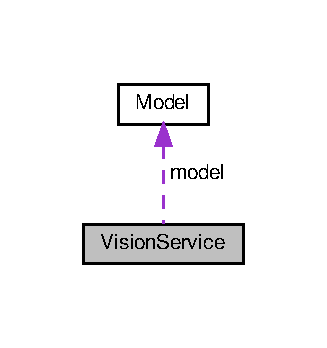
\includegraphics[width=157pt]{classVisionService__coll__graph}
\end{center}
\end{figure}
\subsection*{Public Member Functions}
\begin{DoxyCompactItemize}
\item 
\mbox{\Hypertarget{classVisionService_a40b83115dc945cfa9ed16fdfa3c99ba5}\label{classVisionService_a40b83115dc945cfa9ed16fdfa3c99ba5}} 
bool {\bfseries detect\+Callback} (vision\+::\+Vision\+::\+Request \&, vision\+::\+Vision\+::\+Response \&)
\item 
\mbox{\Hypertarget{classVisionService_a02a14fd32cf867b31c7d711a7b64691f}\label{classVisionService_a02a14fd32cf867b31c7d711a7b64691f}} 
void {\bfseries capture\+Callback} (const sensor\+\_\+msgs\+::\+Image\+Const\+Ptr \&)
\item 
\mbox{\Hypertarget{classVisionService_a1395f4513469c69074c2f7e16da68c13}\label{classVisionService_a1395f4513469c69074c2f7e16da68c13}} 
\hyperlink{structObservation}{Observation} {\bfseries find\+Gate} (const cv\+::\+Mat \&)
\item 
\mbox{\Hypertarget{classVisionService_aa294fde48d52b528ca2082910f7cce2f}\label{classVisionService_aa294fde48d52b528ca2082910f7cce2f}} 
\hyperlink{structObservation}{Observation} {\bfseries find\+Gate\+ML} (cv\+::\+Mat)
\end{DoxyCompactItemize}
\subsection*{Data Fields}
\begin{DoxyCompactItemize}
\item 
\mbox{\Hypertarget{classVisionService_aab2728718c9697f322dc84914a670484}\label{classVisionService_aab2728718c9697f322dc84914a670484}} 
cv\+::\+Mat {\bfseries front}
\item 
\mbox{\Hypertarget{classVisionService_aea4889f5af8acdf4b6e222f67c58477b}\label{classVisionService_aea4889f5af8acdf4b6e222f67c58477b}} 
cv\+::\+Mat {\bfseries down}
\item 
\mbox{\Hypertarget{classVisionService_aa0b7cb339423b293d576e69759a754bc}\label{classVisionService_aa0b7cb339423b293d576e69759a754bc}} 
\hyperlink{classModel}{Model} {\bfseries model}
\item 
\mbox{\Hypertarget{classVisionService_a6089969c6dc3a41dc384b4963f6bd37a}\label{classVisionService_a6089969c6dc3a41dc384b4963f6bd37a}} 
Task {\bfseries task}
\end{DoxyCompactItemize}


The documentation for this class was generated from the following files\+:\begin{DoxyCompactItemize}
\item 
src/sub\+\_\+vision/include/vision/\hyperlink{sub__vision_2include_2vision_2service_8hpp}{service.\+hpp}\item 
src/sub\+\_\+vision/src/\hyperlink{gate_8cpp}{gate.\+cpp}\item 
src/sub\+\_\+vision/src/\hyperlink{sub__vision_2src_2service_8cpp}{service.\+cpp}\end{DoxyCompactItemize}

\chapter{File Documentation}
\hypertarget{atmega_8hpp}{}\section{src/sub\+\_\+control/include/control/atmega.hpp File Reference}
\label{atmega_8hpp}\index{src/sub\+\_\+control/include/control/atmega.\+hpp@{src/sub\+\_\+control/include/control/atmega.\+hpp}}


Function definitions for interfacing with the code on the atmega.  


{\ttfamily \#include \char`\"{}control/state.\+hpp\char`\"{}}\newline
Include dependency graph for atmega.\+hpp\+:\nopagebreak
\begin{figure}[H]
\begin{center}
\leavevmode
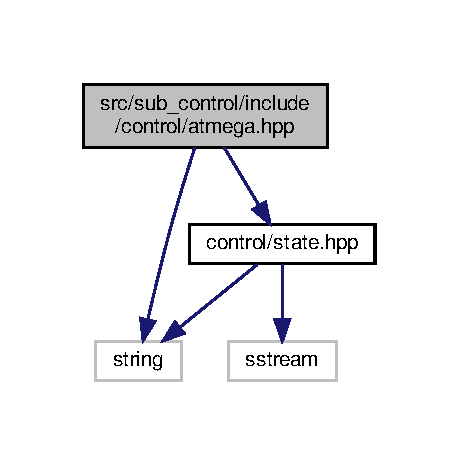
\includegraphics[width=198pt]{atmega_8hpp__incl}
\end{center}
\end{figure}
This graph shows which files directly or indirectly include this file\+:\nopagebreak
\begin{figure}[H]
\begin{center}
\leavevmode
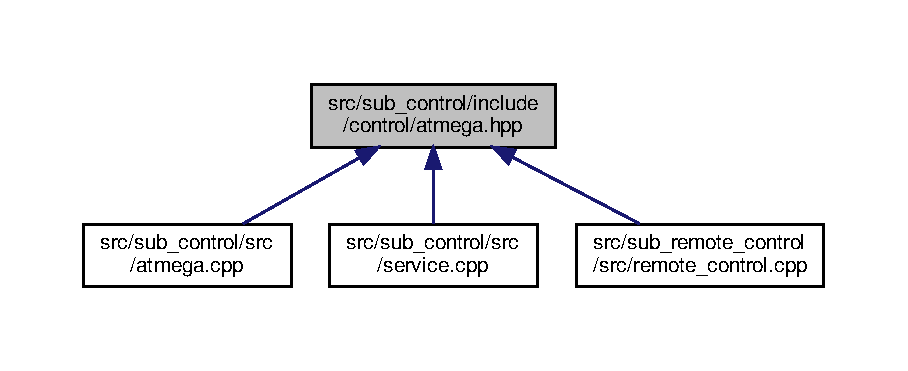
\includegraphics[width=350pt]{atmega_8hpp__dep__incl}
\end{center}
\end{figure}
\subsection*{Macros}
\begin{DoxyCompactItemize}
\item 
\mbox{\Hypertarget{atmega_8hpp_a614217d263be1fb1a5f76e2ff7be19a2}\label{atmega_8hpp_a614217d263be1fb1a5f76e2ff7be19a2}} 
\#define {\bfseries P\+O\+RT}~\char`\"{}/dev/tty\+A\+C\+M0\char`\"{}
\end{DoxyCompactItemize}
\subsection*{Functions}
\begin{DoxyCompactItemize}
\item 
\mbox{\Hypertarget{atmega_8hpp_a8f6680c5d33d6233c25529ff98406679}\label{atmega_8hpp_a8f6680c5d33d6233c25529ff98406679}} 
void {\bfseries atmega\+::write} (std\+::string)
\item 
\mbox{\Hypertarget{atmega_8hpp_a6306408ade4f56d184a373eba5b51922}\label{atmega_8hpp_a6306408ade4f56d184a373eba5b51922}} 
void {\bfseries atmega\+::write} (const \hyperlink{structState}{State} \&)
\item 
\mbox{\Hypertarget{atmega_8hpp_aeba9f31fdbd75c7d289c05ff6ee286c9}\label{atmega_8hpp_aeba9f31fdbd75c7d289c05ff6ee286c9}} 
void {\bfseries atmega\+::relative} (const \hyperlink{structState}{State} \&)
\item 
\mbox{\Hypertarget{atmega_8hpp_a22abb5bf33a5d76d0c31d30185c023bd}\label{atmega_8hpp_a22abb5bf33a5d76d0c31d30185c023bd}} 
bool {\bfseries atmega\+::alive} ()
\item 
\mbox{\Hypertarget{atmega_8hpp_a0cb20880482ecd989647672f6ca2a830}\label{atmega_8hpp_a0cb20880482ecd989647672f6ca2a830}} 
\hyperlink{structState}{State} {\bfseries atmega\+::state} ()
\end{DoxyCompactItemize}
\subsection*{Variables}
\begin{DoxyCompactItemize}
\item 
\mbox{\Hypertarget{atmega_8hpp_a5e34b501678d80ab91465e65389c9749}\label{atmega_8hpp_a5e34b501678d80ab91465e65389c9749}} 
F\+I\+LE $\ast$ {\bfseries atmega\+::in} = fopen(P\+O\+RT, \char`\"{}r+\char`\"{})
\item 
\mbox{\Hypertarget{atmega_8hpp_ae69d979ccfad9a05f9ae8e6c1370585e}\label{atmega_8hpp_ae69d979ccfad9a05f9ae8e6c1370585e}} 
F\+I\+LE $\ast$ {\bfseries atmega\+::out} = fopen(P\+O\+RT, \char`\"{}w+\char`\"{})
\item 
\mbox{\Hypertarget{atmega_8hpp_afa2561d0008822ad2f9a906ab9c7e445}\label{atmega_8hpp_afa2561d0008822ad2f9a906ab9c7e445}} 
\hyperlink{structState}{State} {\bfseries atmega\+::sim\+\_\+state}
\end{DoxyCompactItemize}


\subsection{Detailed Description}
Function definitions for interfacing with the code on the atmega. 

Nothing from mission or vision should depend on this file. Instead, use the control service to ensure that there aren\textquotesingle{}t multiple clients writing to Nautical at the same time.

\begin{DoxyAuthor}{Author}
David Zhang 
\end{DoxyAuthor}

\hypertarget{sub__control_2include_2control_2service_8hpp}{}\section{src/sub\+\_\+control/include/control/service.hpp File Reference}
\label{sub__control_2include_2control_2service_8hpp}\index{src/sub\+\_\+control/include/control/service.\+hpp@{src/sub\+\_\+control/include/control/service.\+hpp}}


Wrapper function definitions for R\+OS services.  


{\ttfamily \#include \char`\"{}control/\+Control\+Alive.\+h\char`\"{}}\newline
{\ttfamily \#include \char`\"{}control/\+Control\+State.\+h\char`\"{}}\newline
{\ttfamily \#include \char`\"{}control/\+Control\+Write.\+h\char`\"{}}\newline
{\ttfamily \#include \char`\"{}control/\+Control\+Write\+State.\+h\char`\"{}}\newline
{\ttfamily \#include \char`\"{}control/\+Control\+Write\+Depth.\+h\char`\"{}}\newline
Include dependency graph for service.\+hpp\+:
\nopagebreak
\begin{figure}[H]
\begin{center}
\leavevmode
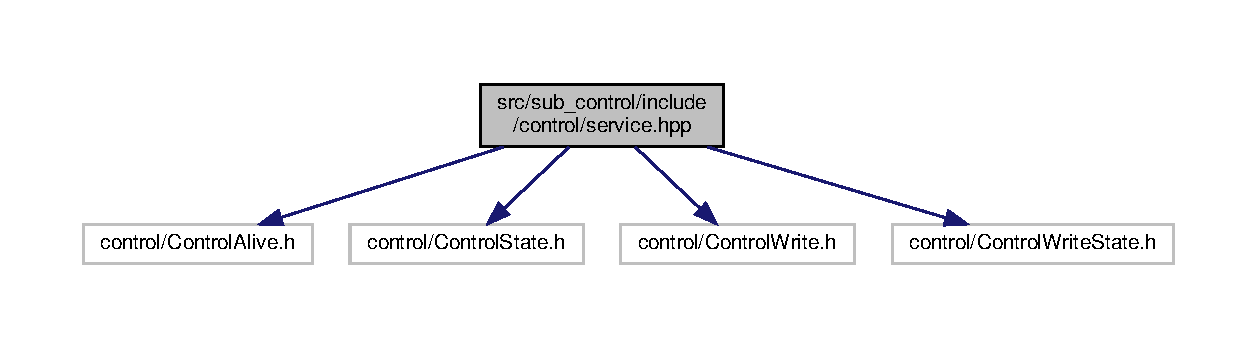
\includegraphics[width=350pt]{sub__control_2include_2control_2service_8hpp__incl}
\end{center}
\end{figure}
This graph shows which files directly or indirectly include this file\+:
\nopagebreak
\begin{figure}[H]
\begin{center}
\leavevmode
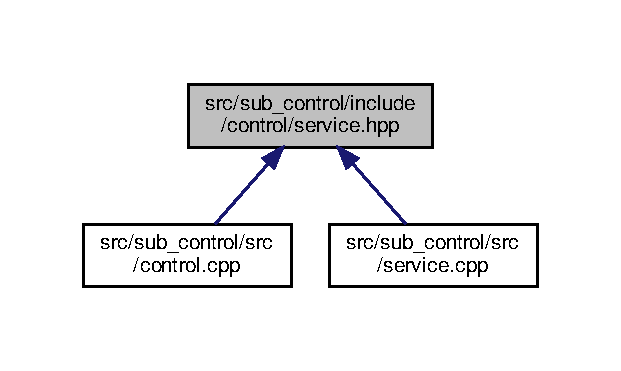
\includegraphics[width=298pt]{sub__control_2include_2control_2service_8hpp__dep__incl}
\end{center}
\end{figure}
\subsection*{Functions}
\begin{DoxyCompactItemize}
\item 
\mbox{\Hypertarget{sub__control_2include_2control_2service_8hpp_aa966962739a88947befa1795953e1b08}\label{sub__control_2include_2control_2service_8hpp_aa966962739a88947befa1795953e1b08}} 
bool {\bfseries alive} (control\+::\+Control\+Alive\+::\+Request \&, control\+::\+Control\+Alive\+::\+Response \&)
\item 
\mbox{\Hypertarget{sub__control_2include_2control_2service_8hpp_a3c691af76571976393934e7830f09ff5}\label{sub__control_2include_2control_2service_8hpp_a3c691af76571976393934e7830f09ff5}} 
bool {\bfseries state} (control\+::\+Control\+State\+::\+Request \&, control\+::\+Control\+State\+::\+Response \&)
\item 
\mbox{\Hypertarget{sub__control_2include_2control_2service_8hpp_a72a9fa525d8cfc7a5aea898d20ad6d80}\label{sub__control_2include_2control_2service_8hpp_a72a9fa525d8cfc7a5aea898d20ad6d80}} 
bool {\bfseries write} (control\+::\+Control\+Write\+::\+Request \&, control\+::\+Control\+Write\+::\+Response \&)
\item 
\mbox{\Hypertarget{sub__control_2include_2control_2service_8hpp_aadc67fe2c1ea7687229ab3331b01368a}\label{sub__control_2include_2control_2service_8hpp_aadc67fe2c1ea7687229ab3331b01368a}} 
bool {\bfseries write\+State} (control\+::\+Control\+Write\+State\+::\+Request \&, control\+::\+Control\+Write\+State\+::\+Response \&)
\item 
\mbox{\Hypertarget{sub__control_2include_2control_2service_8hpp_ade76b4dd0b2f2bf284c14de8296fc757}\label{sub__control_2include_2control_2service_8hpp_ade76b4dd0b2f2bf284c14de8296fc757}} 
bool {\bfseries write\+Depth} (control\+::\+Control\+Write\+Depth\+::\+Request \&, control\+::\+Control\+Write\+Depth\+::\+Response \&)
\end{DoxyCompactItemize}


\subsection{Detailed Description}
Wrapper function definitions for R\+OS services. 

\begin{DoxyAuthor}{Author}
David Zhang 
\end{DoxyAuthor}

\hypertarget{sub__vision_2include_2vision_2service_8hpp}{}\section{src/sub\+\_\+vision/include/vision/service.hpp File Reference}
\label{sub__vision_2include_2vision_2service_8hpp}\index{src/sub\+\_\+vision/include/vision/service.\+hpp@{src/sub\+\_\+vision/include/vision/service.\+hpp}}


Wrapper class to handle the different vision callbacks.  


{\ttfamily \#include $<$ros/ros.\+h$>$}\newline
{\ttfamily \#include $<$image\+\_\+transport/image\+\_\+transport.\+h$>$}\newline
{\ttfamily \#include $<$cv\+\_\+bridge/cv\+\_\+bridge.\+h$>$}\newline
{\ttfamily \#include $<$opencv2/core/core.\+hpp$>$}\newline
{\ttfamily \#include $<$opencv2/highgui/highgui.\+hpp$>$}\newline
{\ttfamily \#include $<$opencv2/imgproc/imgproc.\+hpp$>$}\newline
{\ttfamily \#include $<$vision/\+Vision.\+h$>$}\newline
{\ttfamily \#include \char`\"{}vision/observation.\+hpp\char`\"{}}\newline
{\ttfamily \#include \char`\"{}vision/model.\+hpp\char`\"{}}\newline
{\ttfamily \#include \char`\"{}vision/tensor.\+hpp\char`\"{}}\newline
Include dependency graph for service.\+hpp\+:\nopagebreak
\begin{figure}[H]
\begin{center}
\leavevmode
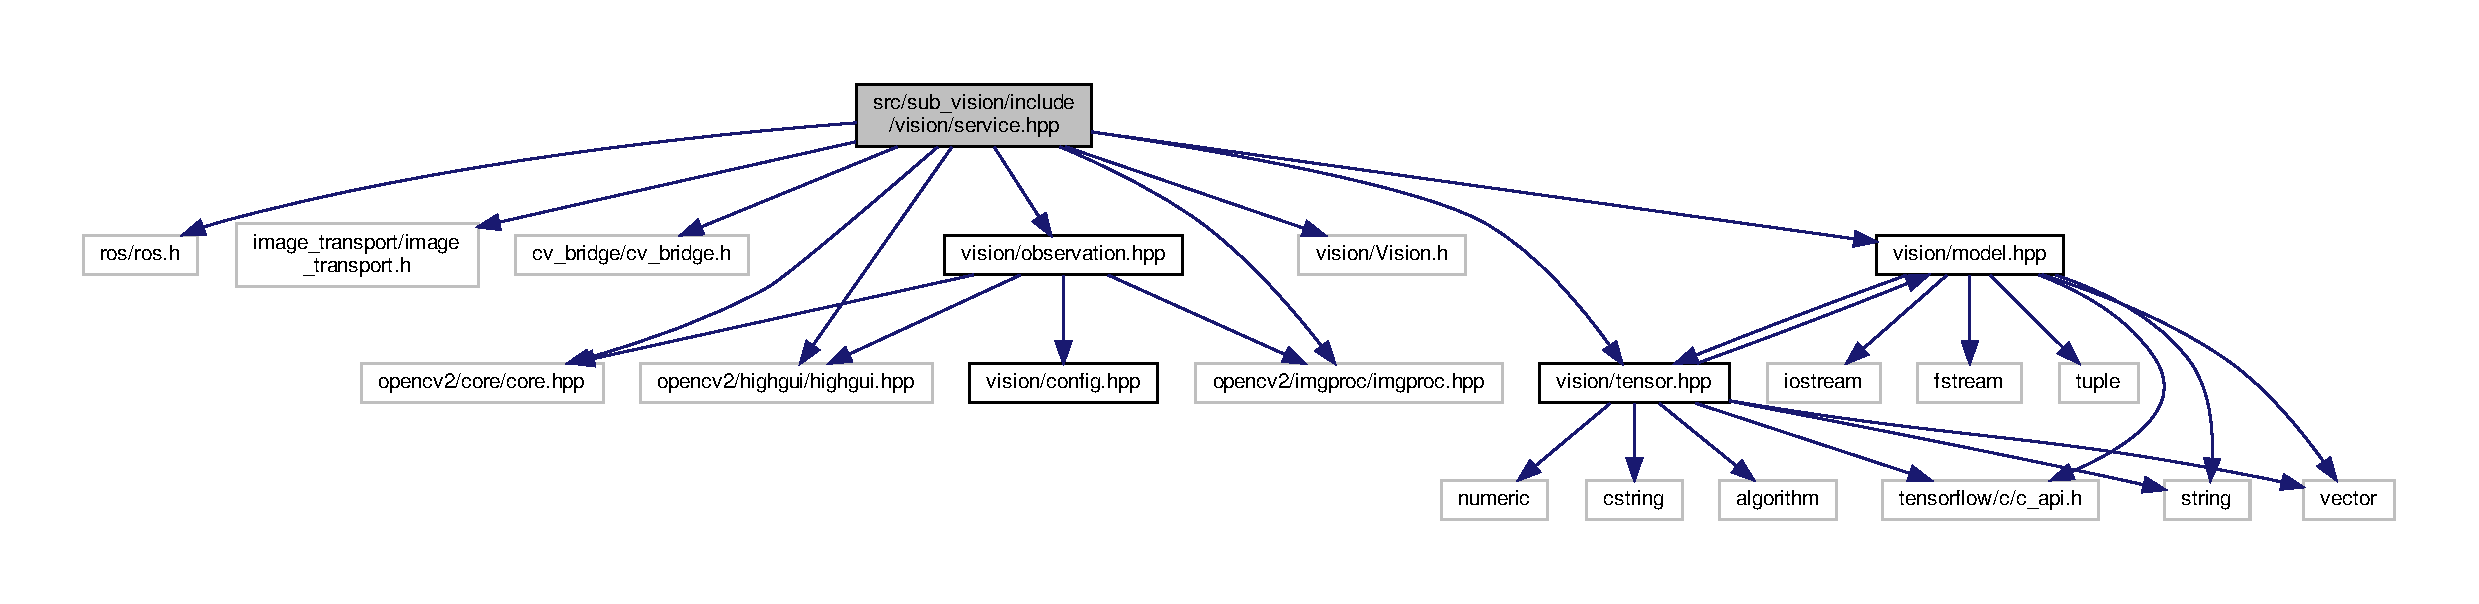
\includegraphics[width=350pt]{sub__vision_2include_2vision_2service_8hpp__incl}
\end{center}
\end{figure}
This graph shows which files directly or indirectly include this file\+:\nopagebreak
\begin{figure}[H]
\begin{center}
\leavevmode
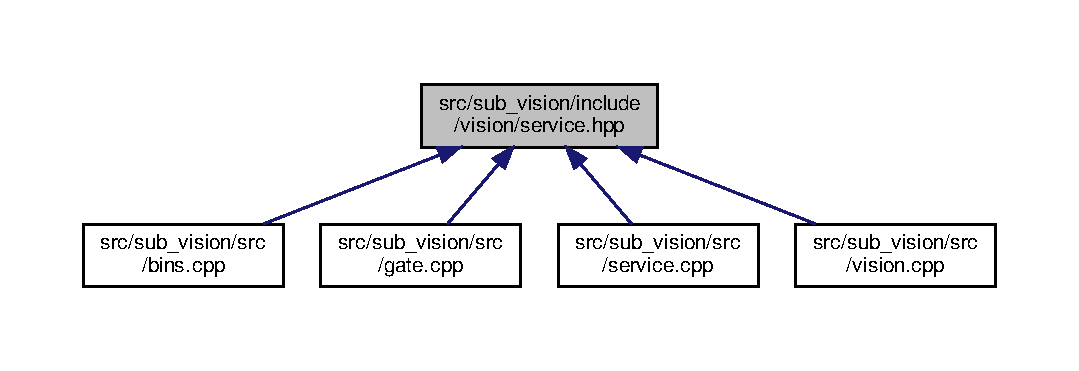
\includegraphics[width=350pt]{sub__vision_2include_2vision_2service_8hpp__dep__incl}
\end{center}
\end{figure}
\subsection*{Data Structures}
\begin{DoxyCompactItemize}
\item 
class \hyperlink{classVisionService}{Vision\+Service}
\end{DoxyCompactItemize}
\subsection*{Functions}
\begin{DoxyCompactItemize}
\item 
\mbox{\Hypertarget{sub__vision_2include_2vision_2service_8hpp_a8b924381d418d87721ce459c31bc8860}\label{sub__vision_2include_2vision_2service_8hpp_a8b924381d418d87721ce459c31bc8860}} 
void {\bfseries set\+Response} (const \hyperlink{structObservation}{Observation} \&, vision\+::\+Vision\+::\+Response \&)
\end{DoxyCompactItemize}


\subsection{Detailed Description}
Wrapper class to handle the different vision callbacks. 

The main purpose of this class is to ensure that the images read from the R\+OS image publisher can be used for object detection. It keeps the images in one location and allows ros\+::spin() to update them as needed.

\begin{DoxyAuthor}{Author}
David Zhang 

Emil Tu 
\end{DoxyAuthor}

\hypertarget{state_8hpp}{}\section{src/sub\+\_\+control/include/control/state.hpp File Reference}
\label{state_8hpp}\index{src/sub\+\_\+control/include/control/state.\+hpp@{src/sub\+\_\+control/include/control/state.\+hpp}}


\hyperlink{structState}{State} struct and constant definitions.  


{\ttfamily \#include $<$string$>$}\newline
{\ttfamily \#include $<$sstream$>$}\newline
Include dependency graph for state.\+hpp\+:\nopagebreak
\begin{figure}[H]
\begin{center}
\leavevmode
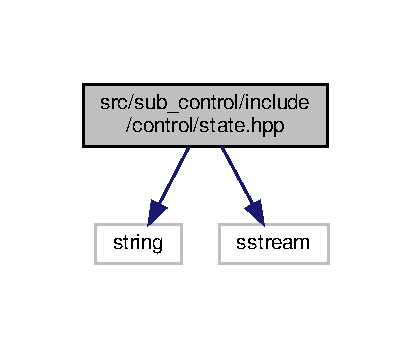
\includegraphics[width=198pt]{state_8hpp__incl}
\end{center}
\end{figure}
This graph shows which files directly or indirectly include this file\+:\nopagebreak
\begin{figure}[H]
\begin{center}
\leavevmode
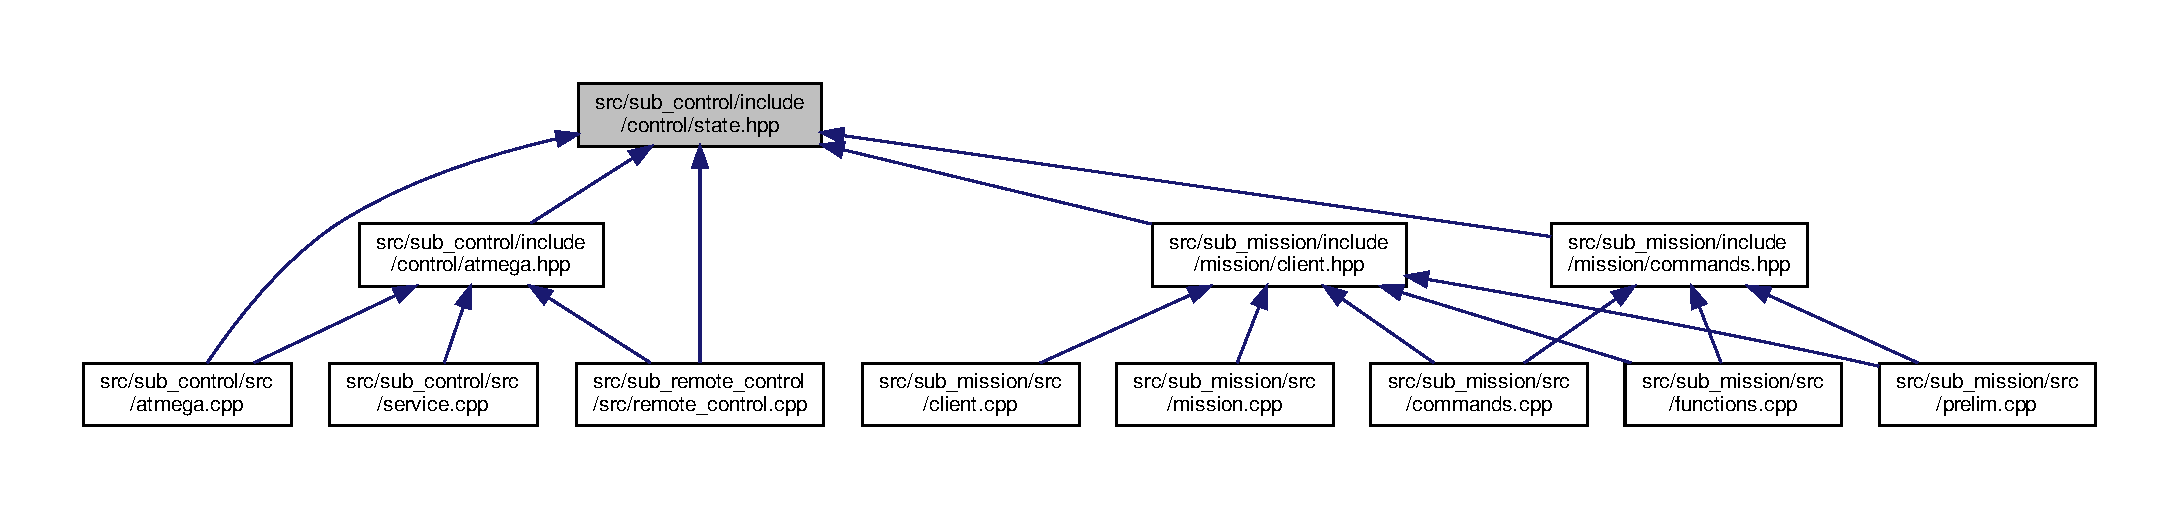
\includegraphics[width=350pt]{state_8hpp__dep__incl}
\end{center}
\end{figure}
\subsection*{Data Structures}
\begin{DoxyCompactItemize}
\item 
struct \hyperlink{structState}{State}
\end{DoxyCompactItemize}
\subsection*{Variables}
\begin{DoxyCompactItemize}
\item 
\mbox{\Hypertarget{state_8hpp_a93188324f4ddec8d3bdac778e12231ba}\label{state_8hpp_a93188324f4ddec8d3bdac778e12231ba}} 
const int {\bfseries X} = 0
\item 
\mbox{\Hypertarget{state_8hpp_a4245f3c5e8eb90ade09427f989b098ec}\label{state_8hpp_a4245f3c5e8eb90ade09427f989b098ec}} 
const int {\bfseries Y} = 1
\item 
\mbox{\Hypertarget{state_8hpp_ad6a5acba3306c0d145b10acd89c52126}\label{state_8hpp_ad6a5acba3306c0d145b10acd89c52126}} 
const int {\bfseries Z} = 2
\item 
\mbox{\Hypertarget{state_8hpp_ae9a1644b752506b32bf480e6966d4f96}\label{state_8hpp_ae9a1644b752506b32bf480e6966d4f96}} 
const int {\bfseries Y\+AW} = 3
\item 
\mbox{\Hypertarget{state_8hpp_af35fbefbfe15684f66cb4c21cfe96a15}\label{state_8hpp_af35fbefbfe15684f66cb4c21cfe96a15}} 
const int {\bfseries P\+I\+T\+CH} = 4
\item 
\mbox{\Hypertarget{state_8hpp_af2837f86c13b08fbdc9827227bde7e20}\label{state_8hpp_af2837f86c13b08fbdc9827227bde7e20}} 
const int {\bfseries R\+O\+LL} = 5
\item 
\mbox{\Hypertarget{state_8hpp_ab2b6b0c222cd1ce70d6a831f57241e59}\label{state_8hpp_ab2b6b0c222cd1ce70d6a831f57241e59}} 
const int {\bfseries N} = 6
\end{DoxyCompactItemize}


\subsection{Detailed Description}
\hyperlink{structState}{State} struct and constant definitions. 

\begin{DoxyAuthor}{Author}
David Zhang 
\end{DoxyAuthor}

\hypertarget{client_8hpp}{}\section{src/sub\+\_\+mission/include/mission/client.hpp File Reference}
\label{client_8hpp}\index{src/sub\+\_\+mission/include/mission/client.\+hpp@{src/sub\+\_\+mission/include/mission/client.\+hpp}}


Wrapper namespaces for using R\+OS clients.  


{\ttfamily \#include $<$ros/ros.\+h$>$}\newline
{\ttfamily \#include $<$control/\+Control\+Alive.\+h$>$}\newline
{\ttfamily \#include $<$control/\+Control\+State.\+h$>$}\newline
{\ttfamily \#include $<$control/\+Control\+Write.\+h$>$}\newline
{\ttfamily \#include $<$control/\+Control\+Write\+State.\+h$>$}\newline
{\ttfamily \#include $<$control/\+Control\+Write\+Depth.\+h$>$}\newline
{\ttfamily \#include $<$vision/\+Vision.\+h$>$}\newline
{\ttfamily \#include \char`\"{}control/state.\+hpp\char`\"{}}\newline
{\ttfamily \#include \char`\"{}vision/observation.\+hpp\char`\"{}}\newline
Include dependency graph for client.\+hpp\+:
\nopagebreak
\begin{figure}[H]
\begin{center}
\leavevmode
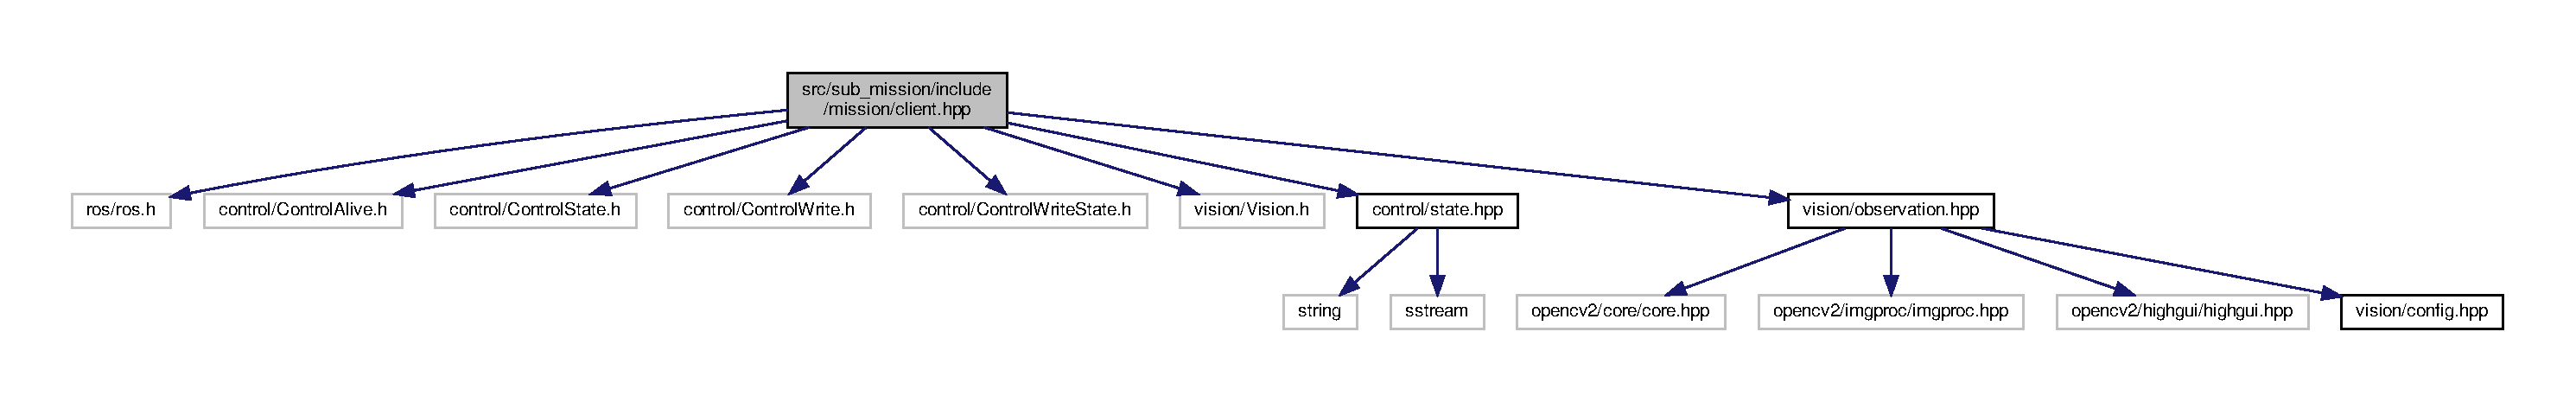
\includegraphics[width=350pt]{client_8hpp__incl}
\end{center}
\end{figure}
This graph shows which files directly or indirectly include this file\+:
\nopagebreak
\begin{figure}[H]
\begin{center}
\leavevmode
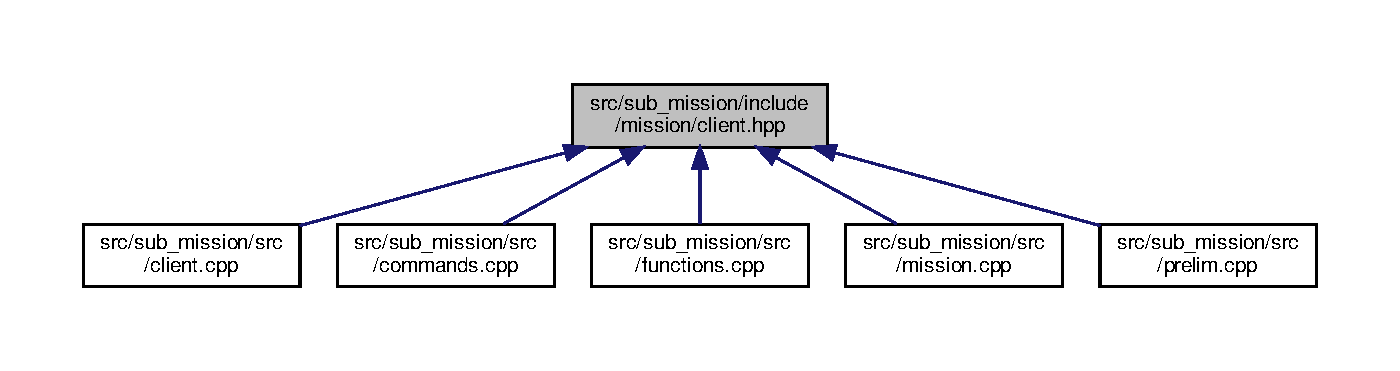
\includegraphics[width=350pt]{client_8hpp__dep__incl}
\end{center}
\end{figure}
\subsection*{Functions}
\begin{DoxyCompactItemize}
\item 
\mbox{\Hypertarget{client_8hpp_afcc2ae7b458f182fb618080fb06e8221}\label{client_8hpp_afcc2ae7b458f182fb618080fb06e8221}} 
\hyperlink{structObservation}{Observation} {\bfseries vision\+\_\+client\+::vision} (Task, int)
\item 
\mbox{\Hypertarget{client_8hpp_a3ded3efee9af8fa3b086be935dd60342}\label{client_8hpp_a3ded3efee9af8fa3b086be935dd60342}} 
bool {\bfseries control\+\_\+client\+::alive} ()
\item 
\mbox{\Hypertarget{client_8hpp_a75378d18ff05eaadffa1c9a2c3a5ec59}\label{client_8hpp_a75378d18ff05eaadffa1c9a2c3a5ec59}} 
\hyperlink{structState}{State} {\bfseries control\+\_\+client\+::state} ()
\item 
\mbox{\Hypertarget{client_8hpp_a115f3dde3379c8578b98935367722193}\label{client_8hpp_a115f3dde3379c8578b98935367722193}} 
void {\bfseries control\+\_\+client\+::write} (std\+::string)
\item 
\mbox{\Hypertarget{client_8hpp_ae5b5378396735164a81dfb5650332d56}\label{client_8hpp_ae5b5378396735164a81dfb5650332d56}} 
void {\bfseries control\+\_\+client\+::write\+State} (const \hyperlink{structState}{State} \&)
\item 
\mbox{\Hypertarget{client_8hpp_a2033407e86ac3be6f3ca6ea6e97d0d0a}\label{client_8hpp_a2033407e86ac3be6f3ca6ea6e97d0d0a}} 
void {\bfseries control\+\_\+client\+::write\+Depth} (float)
\end{DoxyCompactItemize}
\subsection*{Variables}
\begin{DoxyCompactItemize}
\item 
\mbox{\Hypertarget{client_8hpp_a4e91512e5fb519f996fc33db995ce976}\label{client_8hpp_a4e91512e5fb519f996fc33db995ce976}} 
ros\+::\+Service\+Client {\bfseries vision\+\_\+client\+::client}
\item 
\mbox{\Hypertarget{client_8hpp_ac0be764f14f7a4154db3baf1c77f887c}\label{client_8hpp_ac0be764f14f7a4154db3baf1c77f887c}} 
ros\+::\+Service\+Client {\bfseries control\+\_\+client\+::alive\+\_\+client}
\item 
\mbox{\Hypertarget{client_8hpp_a49c5331ba74813000221f2cafaca72f7}\label{client_8hpp_a49c5331ba74813000221f2cafaca72f7}} 
ros\+::\+Service\+Client {\bfseries control\+\_\+client\+::state\+\_\+client}
\item 
\mbox{\Hypertarget{client_8hpp_a919659ad17d351d0066a8cc3e1b90d45}\label{client_8hpp_a919659ad17d351d0066a8cc3e1b90d45}} 
ros\+::\+Service\+Client {\bfseries control\+\_\+client\+::write\+\_\+client}
\item 
\mbox{\Hypertarget{client_8hpp_a86f1dd68b90c714865ec38c5ffe4e367}\label{client_8hpp_a86f1dd68b90c714865ec38c5ffe4e367}} 
ros\+::\+Service\+Client {\bfseries control\+\_\+client\+::write\+\_\+state\+\_\+client}
\item 
\mbox{\Hypertarget{client_8hpp_a4badc54a75589d24181b7ac25deedbd3}\label{client_8hpp_a4badc54a75589d24181b7ac25deedbd3}} 
ros\+::\+Service\+Client {\bfseries control\+\_\+client\+::write\+\_\+depth\+\_\+client}
\end{DoxyCompactItemize}


\subsection{Detailed Description}
Wrapper namespaces for using R\+OS clients. 

\begin{DoxyAuthor}{Author}
David Zhang 
\end{DoxyAuthor}

\hypertarget{commands_8hpp}{}\section{src/sub\+\_\+mission/include/mission/commands.hpp File Reference}
\label{commands_8hpp}\index{src/sub\+\_\+mission/include/mission/commands.\+hpp@{src/sub\+\_\+mission/include/mission/commands.\+hpp}}


Function definitions for generic competition actions.  


{\ttfamily \#include $<$tuple$>$}\newline
{\ttfamily \#include $<$ros/ros.\+h$>$}\newline
{\ttfamily \#include $<$vision/\+Vision.\+h$>$}\newline
{\ttfamily \#include \char`\"{}control/state.\+hpp\char`\"{}}\newline
{\ttfamily \#include \char`\"{}vision/observation.\+hpp\char`\"{}}\newline
Include dependency graph for commands.\+hpp\+:
\nopagebreak
\begin{figure}[H]
\begin{center}
\leavevmode
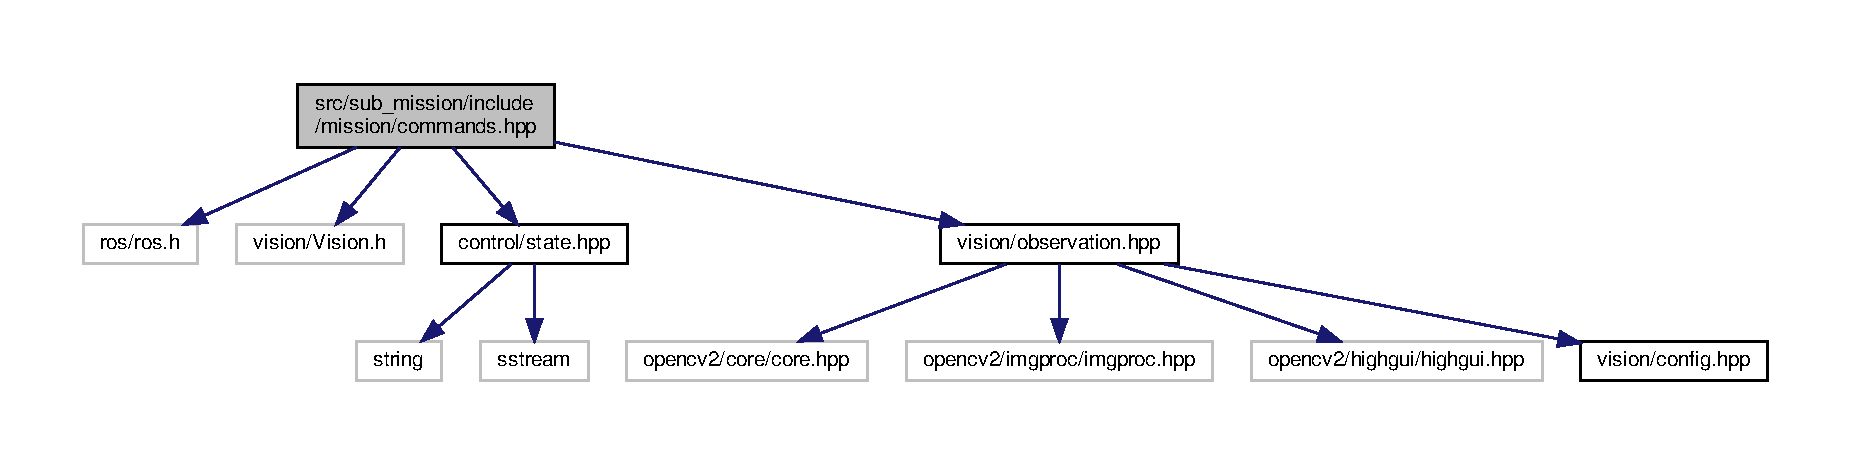
\includegraphics[width=350pt]{commands_8hpp__incl}
\end{center}
\end{figure}
This graph shows which files directly or indirectly include this file\+:
\nopagebreak
\begin{figure}[H]
\begin{center}
\leavevmode
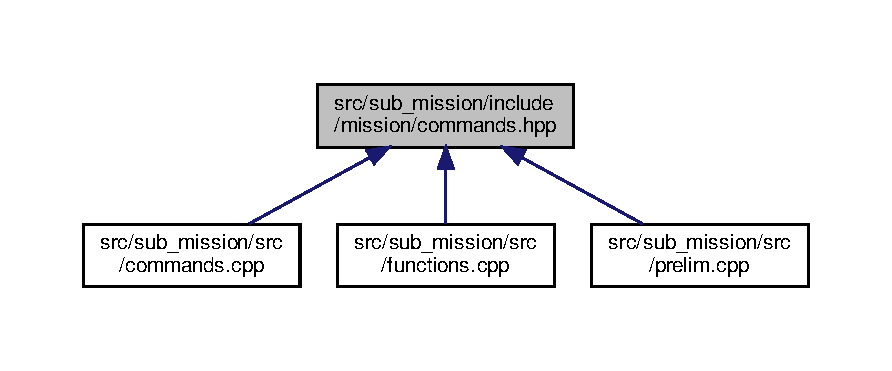
\includegraphics[width=350pt]{commands_8hpp__dep__incl}
\end{center}
\end{figure}
\subsection*{Functions}
\begin{DoxyCompactItemize}
\item 
\mbox{\Hypertarget{commands_8hpp_aae4d42d26c0351a68c7af7cdfbd96798}\label{commands_8hpp_aae4d42d26c0351a68c7af7cdfbd96798}} 
float {\bfseries align} (int, Task, int)
\item 
\mbox{\Hypertarget{commands_8hpp_a3a845107a07d26b3fcde5fb75deb7ccb}\label{commands_8hpp_a3a845107a07d26b3fcde5fb75deb7ccb}} 
std\+::pair$<$ float, float $>$ {\bfseries down\+\_\+align} (int, float, Task, int)
\item 
\mbox{\Hypertarget{commands_8hpp_ab558e6d0f7ffc29c227d195d0ad0f5aa}\label{commands_8hpp_ab558e6d0f7ffc29c227d195d0ad0f5aa}} 
void {\bfseries move} (const \hyperlink{structState}{State} \&)
\end{DoxyCompactItemize}


\subsection{Detailed Description}
Function definitions for generic competition actions. 

\begin{DoxyAuthor}{Author}
David Zhang 
\end{DoxyAuthor}

\hypertarget{functions_8hpp}{}\section{src/sub\+\_\+mission/include/mission/functions.hpp File Reference}
\label{functions_8hpp}\index{src/sub\+\_\+mission/include/mission/functions.\+hpp@{src/sub\+\_\+mission/include/mission/functions.\+hpp}}


Function definitions for each task process during competition.  


{\ttfamily \#include $<$ros/ros.\+h$>$}\newline
{\ttfamily \#include $<$vision/\+Vision.\+h$>$}\newline
Include dependency graph for functions.\+hpp\+:\nopagebreak
\begin{figure}[H]
\begin{center}
\leavevmode
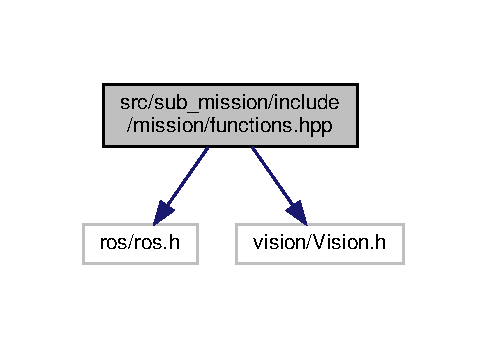
\includegraphics[width=234pt]{functions_8hpp__incl}
\end{center}
\end{figure}
\subsection*{Functions}
\begin{DoxyCompactItemize}
\item 
\mbox{\Hypertarget{functions_8hpp_ae7720475b16624848b395c7eb63bed08}\label{functions_8hpp_ae7720475b16624848b395c7eb63bed08}} 
void {\bfseries gate} ()
\item 
\mbox{\Hypertarget{functions_8hpp_a09f09f738e5df05de88dc2b381cc3346}\label{functions_8hpp_a09f09f738e5df05de88dc2b381cc3346}} 
void {\bfseries octagon} ()
\end{DoxyCompactItemize}


\subsection{Detailed Description}
Function definitions for each task process during competition. 

\begin{DoxyAuthor}{Author}
David Zhang 
\end{DoxyAuthor}

\hypertarget{camera_8hpp}{}\section{src/sub\+\_\+vision/include/vision/camera.hpp File Reference}
\label{camera_8hpp}\index{src/sub\+\_\+vision/include/vision/camera.\+hpp@{src/sub\+\_\+vision/include/vision/camera.\+hpp}}


\hyperlink{structCamera}{Camera} struct for Fly\+Capture based cameras.  


{\ttfamily \#include $<$opencv2/core/core.\+hpp$>$}\newline
{\ttfamily \#include $<$flycapture/\+Fly\+Capture2.\+h$>$}\newline
Include dependency graph for camera.\+hpp\+:\nopagebreak
\begin{figure}[H]
\begin{center}
\leavevmode
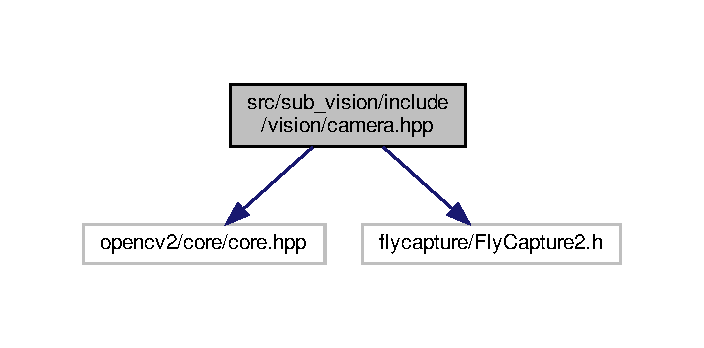
\includegraphics[width=338pt]{camera_8hpp__incl}
\end{center}
\end{figure}
This graph shows which files directly or indirectly include this file\+:\nopagebreak
\begin{figure}[H]
\begin{center}
\leavevmode
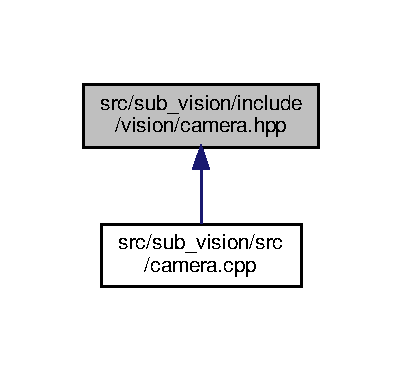
\includegraphics[width=290pt]{camera_8hpp__dep__incl}
\end{center}
\end{figure}
\subsection*{Data Structures}
\begin{DoxyCompactItemize}
\item 
struct \hyperlink{structCamera}{Camera}
\end{DoxyCompactItemize}


\subsection{Detailed Description}
\hyperlink{structCamera}{Camera} struct for Fly\+Capture based cameras. 

\begin{DoxyAuthor}{Author}
Surya Ramesh 
\end{DoxyAuthor}

\hypertarget{config_8hpp}{}\section{src/sub\+\_\+vision/include/vision/config.hpp File Reference}
\label{config_8hpp}\index{src/sub\+\_\+vision/include/vision/config.\+hpp@{src/sub\+\_\+vision/include/vision/config.\+hpp}}


Vision configuration that is used in other packages as well.  


This graph shows which files directly or indirectly include this file\+:\nopagebreak
\begin{figure}[H]
\begin{center}
\leavevmode
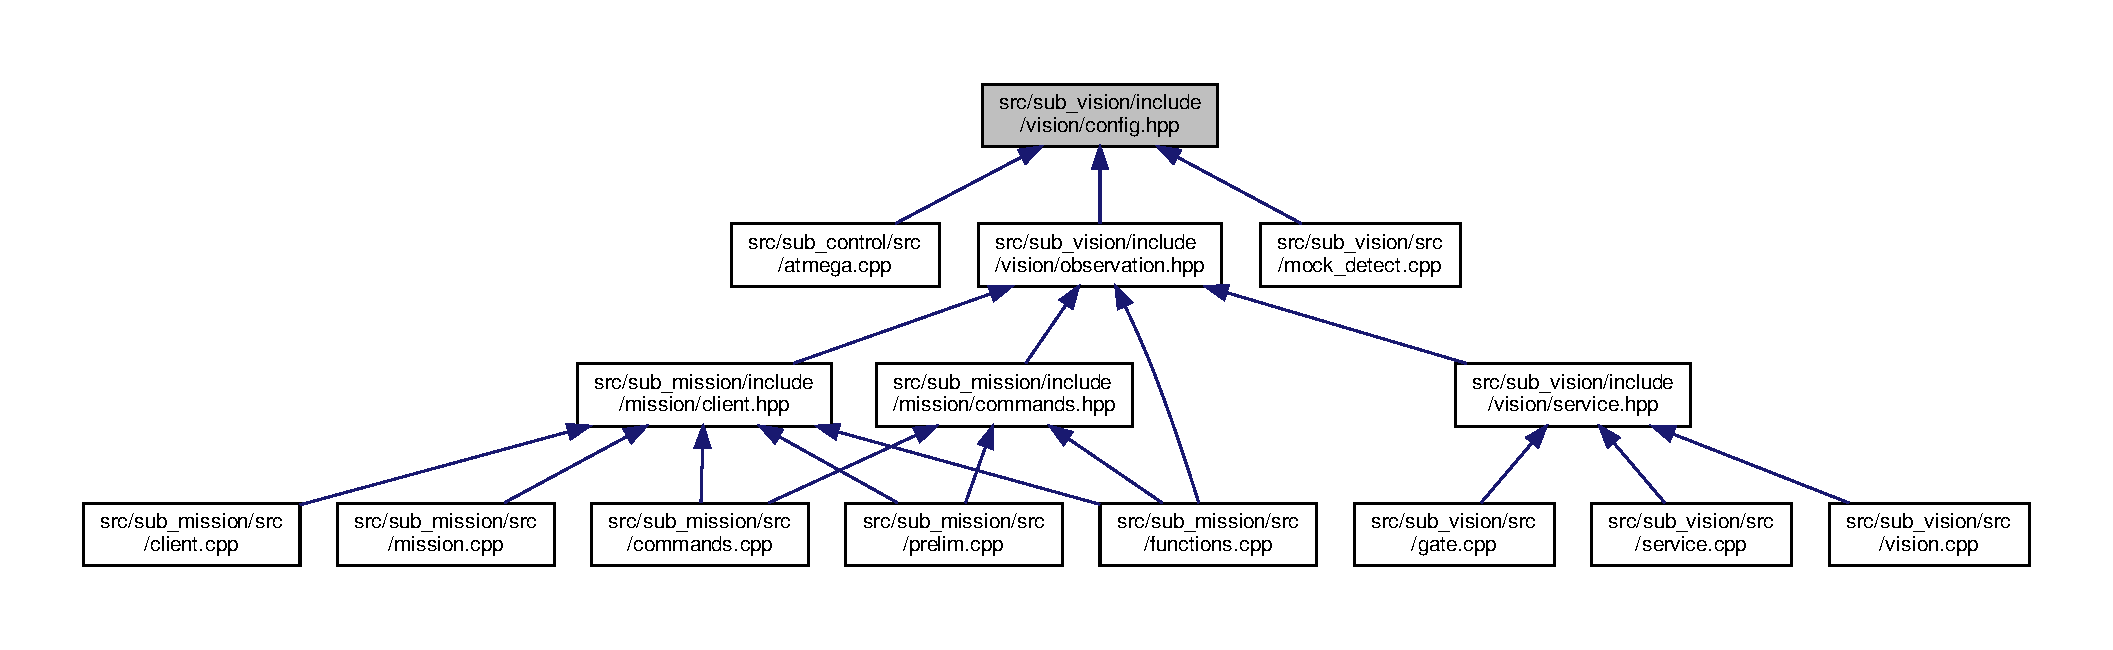
\includegraphics[width=350pt]{config_8hpp__dep__incl}
\end{center}
\end{figure}
\subsection*{Enumerations}
\begin{DoxyCompactItemize}
\item 
\mbox{\Hypertarget{config_8hpp_ac6e73fe6ce68e10b0acd6d2312bdbb35}\label{config_8hpp_ac6e73fe6ce68e10b0acd6d2312bdbb35}} 
enum {\bfseries Camera\+Mode} \{ {\bfseries M\+O\+CK}, 
{\bfseries L\+I\+VE}
 \}
\item 
\mbox{\Hypertarget{config_8hpp_a8564c478026655cd8718601a4514e1b7}\label{config_8hpp_a8564c478026655cd8718601a4514e1b7}} 
enum {\bfseries Task} \{ {\bfseries N\+O\+NE}, 
{\bfseries G\+A\+TE}, 
{\bfseries G\+A\+T\+E\+\_\+\+ML}, 
{\bfseries O\+C\+T\+A\+G\+ON}
 \}
\end{DoxyCompactItemize}
\subsection*{Variables}
\begin{DoxyCompactItemize}
\item 
\mbox{\Hypertarget{config_8hpp_ac47fa8bc6271df01fb9523aab4462b38}\label{config_8hpp_ac47fa8bc6271df01fb9523aab4462b38}} 
const Camera\+Mode {\bfseries C\+A\+M\+E\+R\+A\+\_\+\+M\+O\+DE} = Camera\+Mode\+::\+L\+I\+VE
\item 
\mbox{\Hypertarget{config_8hpp_a6f0eea21585da0907cee0edf287ff4e7}\label{config_8hpp_a6f0eea21585da0907cee0edf287ff4e7}} 
const bool {\bfseries L\+OG} = true
\item 
\mbox{\Hypertarget{config_8hpp_aa46038f18b052a45acb16d3f04e3a947}\label{config_8hpp_aa46038f18b052a45acb16d3f04e3a947}} 
const float {\bfseries H\+F\+OV} = 83
\item 
\mbox{\Hypertarget{config_8hpp_a6e9845852cf8150b694f3dcb5f2ff4a9}\label{config_8hpp_a6e9845852cf8150b694f3dcb5f2ff4a9}} 
const float {\bfseries V\+F\+OV} = 90
\item 
\mbox{\Hypertarget{config_8hpp_a74b36851d26bfffaded0029d686e7421}\label{config_8hpp_a74b36851d26bfffaded0029d686e7421}} 
const int {\bfseries F\+R\+O\+NT} = 0
\item 
\mbox{\Hypertarget{config_8hpp_a434e4725f04fa366ed1341f04d38521d}\label{config_8hpp_a434e4725f04fa366ed1341f04d38521d}} 
const int {\bfseries D\+O\+WN} = 1
\item 
\mbox{\Hypertarget{config_8hpp_abe871fe2aeffb124888d25e08184b01b}\label{config_8hpp_abe871fe2aeffb124888d25e08184b01b}} 
const float {\bfseries F\+I\+M\+G\+\_\+\+D\+IM} \mbox{[}2\mbox{]} = \{ 3648, 5472 \}
\item 
\mbox{\Hypertarget{config_8hpp_a479f30bcb1bd75d0879caac76f69ee39}\label{config_8hpp_a479f30bcb1bd75d0879caac76f69ee39}} 
const float {\bfseries D\+I\+M\+G\+\_\+\+D\+IM} \mbox{[}2\mbox{]} = \{ 480, 640 \}
\end{DoxyCompactItemize}


\subsection{Detailed Description}
Vision configuration that is used in other packages as well. 

\begin{DoxyAuthor}{Author}
David Zhang 
\end{DoxyAuthor}

\hypertarget{filters_8hpp}{}\section{src/sub\+\_\+vision/include/vision/filters.hpp File Reference}
\label{filters_8hpp}\index{src/sub\+\_\+vision/include/vision/filters.\+hpp@{src/sub\+\_\+vision/include/vision/filters.\+hpp}}


Vision filtering function definitions.  


{\ttfamily \#include $<$opencv2/core/core.\+hpp$>$}\newline
{\ttfamily \#include $<$opencv2/imgproc/imgproc.\+hpp$>$}\newline
Include dependency graph for filters.\+hpp\+:\nopagebreak
\begin{figure}[H]
\begin{center}
\leavevmode
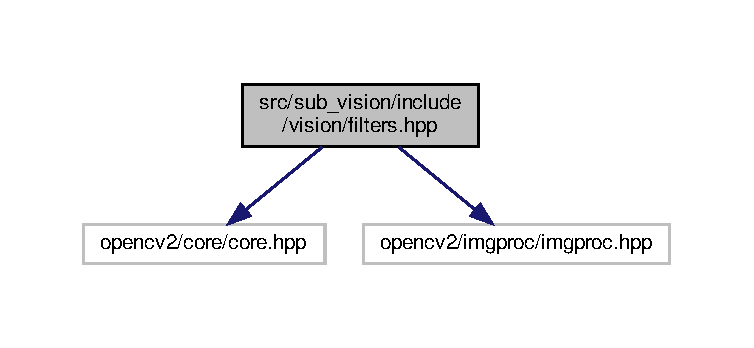
\includegraphics[width=350pt]{filters_8hpp__incl}
\end{center}
\end{figure}
This graph shows which files directly or indirectly include this file\+:\nopagebreak
\begin{figure}[H]
\begin{center}
\leavevmode
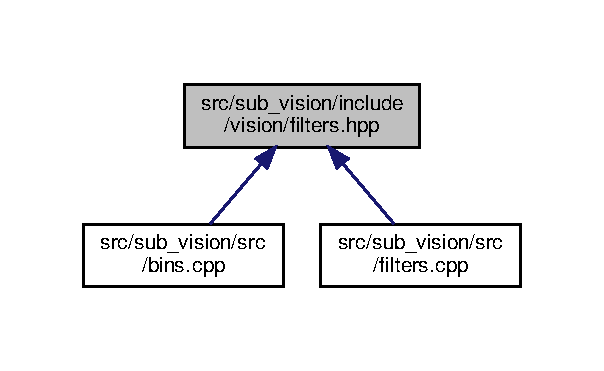
\includegraphics[width=350pt]{filters_8hpp__dep__incl}
\end{center}
\end{figure}
\subsection*{Functions}
\begin{DoxyCompactItemize}
\item 
\mbox{\Hypertarget{filters_8hpp_ae5228b9d44105d900fdd98b30dd7086e}\label{filters_8hpp_ae5228b9d44105d900fdd98b30dd7086e}} 
cv\+::\+Mat {\bfseries equalize\+Hist} (bool, bool, bool, const cv\+::\+Mat \&)
\item 
\mbox{\Hypertarget{filters_8hpp_a71aa95a0c608e22a875d86a22364b6f3}\label{filters_8hpp_a71aa95a0c608e22a875d86a22364b6f3}} 
cv\+::\+Mat {\bfseries illumination} (const cv\+::\+Mat \&)
\item 
\mbox{\Hypertarget{filters_8hpp_a23c0af96549c4cdd5dc452dd987b5817}\label{filters_8hpp_a23c0af96549c4cdd5dc452dd987b5817}} 
cv\+::\+Mat {\bfseries homomorphic} (const cv\+::\+Mat \&)
\item 
\mbox{\Hypertarget{filters_8hpp_a2666eccbbbd045b8554b974b86bdf99c}\label{filters_8hpp_a2666eccbbbd045b8554b974b86bdf99c}} 
cv\+::\+Mat {\bfseries butterworth} (const cv\+::\+Mat \&, int, int, int, int)
\item 
\mbox{\Hypertarget{filters_8hpp_ad6e666ba4519fa51359a7e88492772cb}\label{filters_8hpp_ad6e666ba4519fa51359a7e88492772cb}} 
void {\bfseries fft} (const cv\+::\+Mat \&, cv\+::\+Mat \&)
\end{DoxyCompactItemize}


\subsection{Detailed Description}
Vision filtering function definitions. 

\begin{DoxyAuthor}{Author}
David Zhang 

Arnav Garg 
\end{DoxyAuthor}

\hypertarget{log_8hpp}{}\section{src/sub\+\_\+vision/include/vision/log.hpp File Reference}
\label{log_8hpp}\index{src/sub\+\_\+vision/include/vision/log.\+hpp@{src/sub\+\_\+vision/include/vision/log.\+hpp}}


Logging function definitions for images or text.  


{\ttfamily \#include $<$opencv2/core/core.\+hpp$>$}\newline
{\ttfamily \#include $<$opencv2/highgui/highgui.\+hpp$>$}\newline
{\ttfamily \#include $<$opencv2/imgproc/imgproc.\+hpp$>$}\newline
Include dependency graph for log.\+hpp\+:\nopagebreak
\begin{figure}[H]
\begin{center}
\leavevmode
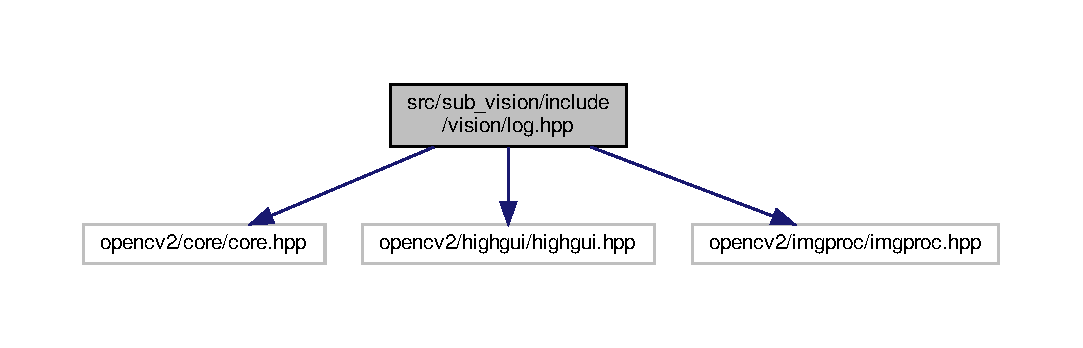
\includegraphics[width=350pt]{log_8hpp__incl}
\end{center}
\end{figure}
This graph shows which files directly or indirectly include this file\+:
\nopagebreak
\begin{figure}[H]
\begin{center}
\leavevmode
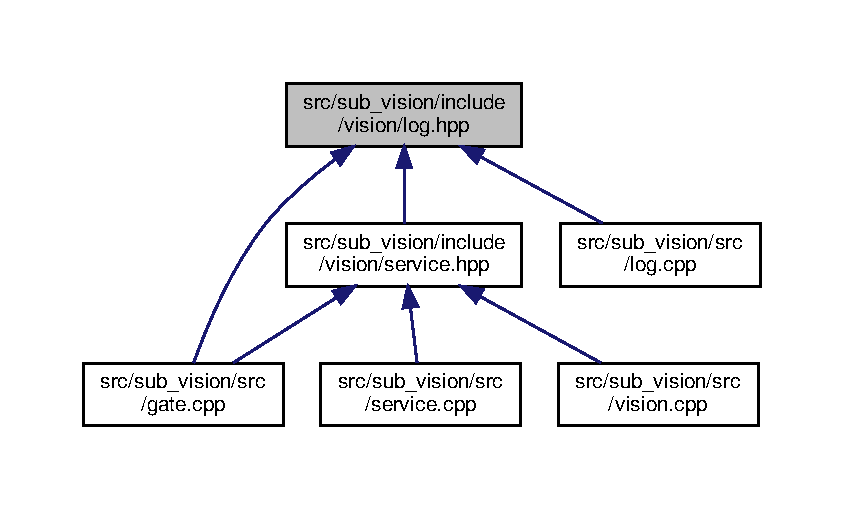
\includegraphics[width=350pt]{log_8hpp__dep__incl}
\end{center}
\end{figure}
\subsection*{Functions}
\begin{DoxyCompactItemize}
\item 
\mbox{\Hypertarget{log_8hpp_a8b9fe1cbfc2c2f234306735834094261}\label{log_8hpp_a8b9fe1cbfc2c2f234306735834094261}} 
void {\bfseries log} (const cv\+::\+Mat \&, char ending)
\item 
\mbox{\Hypertarget{log_8hpp_a02fd73d861ef2e4aabb38c0c9ff82947}\label{log_8hpp_a02fd73d861ef2e4aabb38c0c9ff82947}} 
void {\bfseries init} ()
\end{DoxyCompactItemize}


\subsection{Detailed Description}
Logging function definitions for images or text. 

\begin{DoxyAuthor}{Author}
David Zhang 
\end{DoxyAuthor}

\hypertarget{model_8hpp}{}\section{src/sub\+\_\+vision/include/vision/model.hpp File Reference}
\label{model_8hpp}\index{src/sub\+\_\+vision/include/vision/model.\+hpp@{src/sub\+\_\+vision/include/vision/model.\+hpp}}


TF Object Detection A\+PI C++ wrapper for models.  


{\ttfamily \#include $<$tensorflow/c/c\+\_\+api.\+h$>$}\newline
{\ttfamily \#include $<$string$>$}\newline
{\ttfamily \#include $<$vector$>$}\newline
{\ttfamily \#include $<$iostream$>$}\newline
{\ttfamily \#include $<$fstream$>$}\newline
{\ttfamily \#include $<$tuple$>$}\newline
{\ttfamily \#include \char`\"{}vision/tensor.\+hpp\char`\"{}}\newline
Include dependency graph for model.\+hpp\+:\nopagebreak
\begin{figure}[H]
\begin{center}
\leavevmode
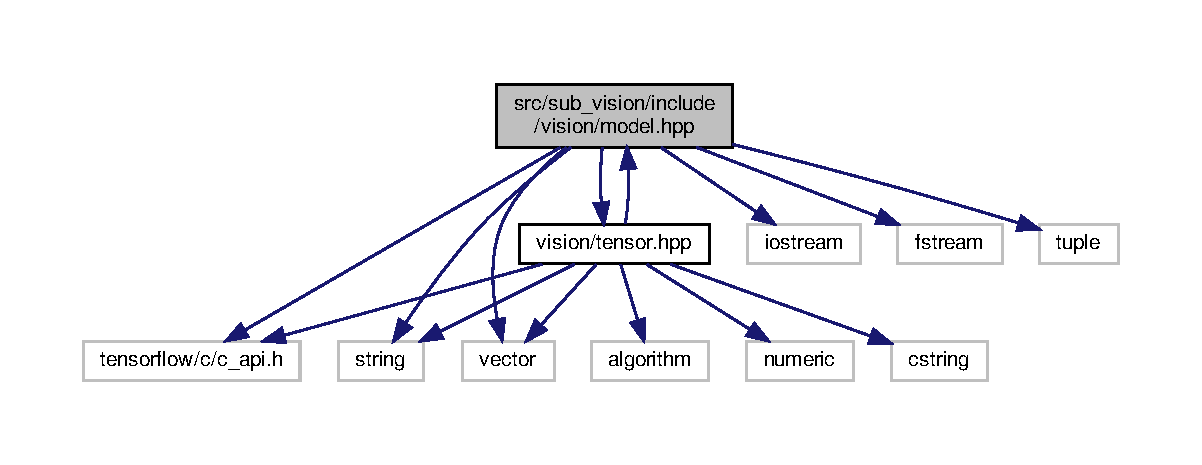
\includegraphics[width=350pt]{model_8hpp__incl}
\end{center}
\end{figure}
This graph shows which files directly or indirectly include this file\+:
\nopagebreak
\begin{figure}[H]
\begin{center}
\leavevmode
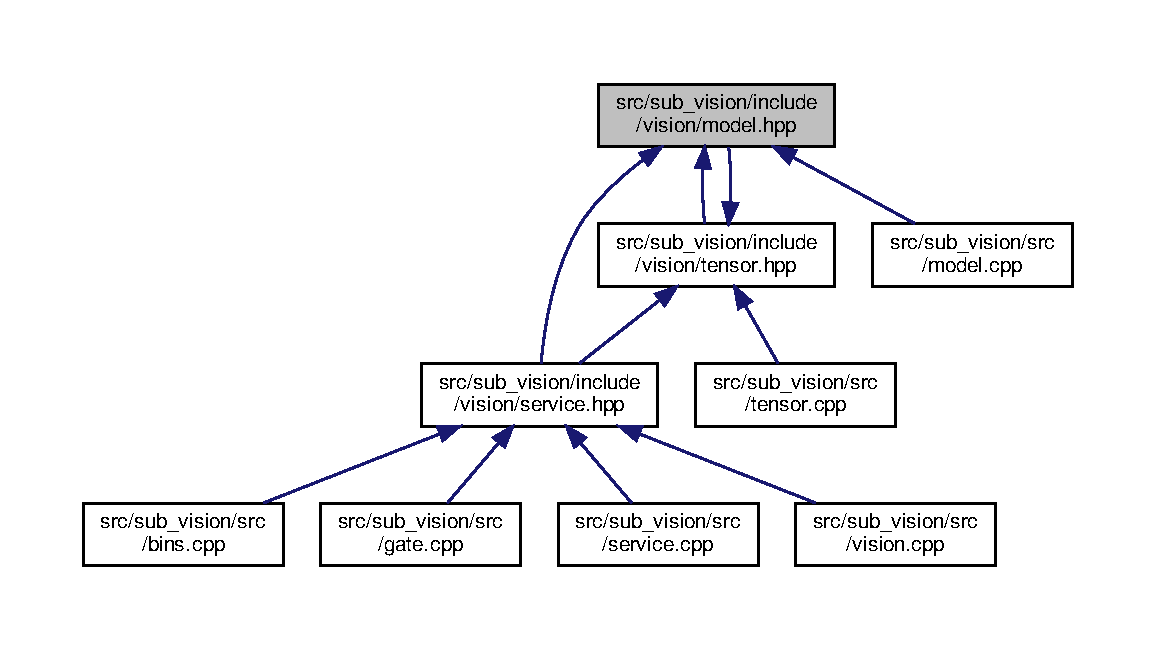
\includegraphics[width=350pt]{model_8hpp__dep__incl}
\end{center}
\end{figure}
\subsection*{Data Structures}
\begin{DoxyCompactItemize}
\item 
class \hyperlink{classModel}{Model}
\end{DoxyCompactItemize}


\subsection{Detailed Description}
TF Object Detection A\+PI C++ wrapper for models. 

\begin{DoxyAuthor}{Author}
Sergio Izquierdo 
\end{DoxyAuthor}

\hypertarget{observation_8hpp}{}\section{src/sub\+\_\+vision/include/vision/observation.hpp File Reference}
\label{observation_8hpp}\index{src/sub\+\_\+vision/include/vision/observation.\+hpp@{src/sub\+\_\+vision/include/vision/observation.\+hpp}}


\hyperlink{structObservation}{Observation} struct definition that represents the results from an object detection function.  


{\ttfamily \#include $<$opencv2/core/core.\+hpp$>$}\newline
{\ttfamily \#include $<$opencv2/imgproc/imgproc.\+hpp$>$}\newline
{\ttfamily \#include $<$opencv2/highgui/highgui.\+hpp$>$}\newline
{\ttfamily \#include \char`\"{}vision/config.\+hpp\char`\"{}}\newline
Include dependency graph for observation.\+hpp\+:\nopagebreak
\begin{figure}[H]
\begin{center}
\leavevmode
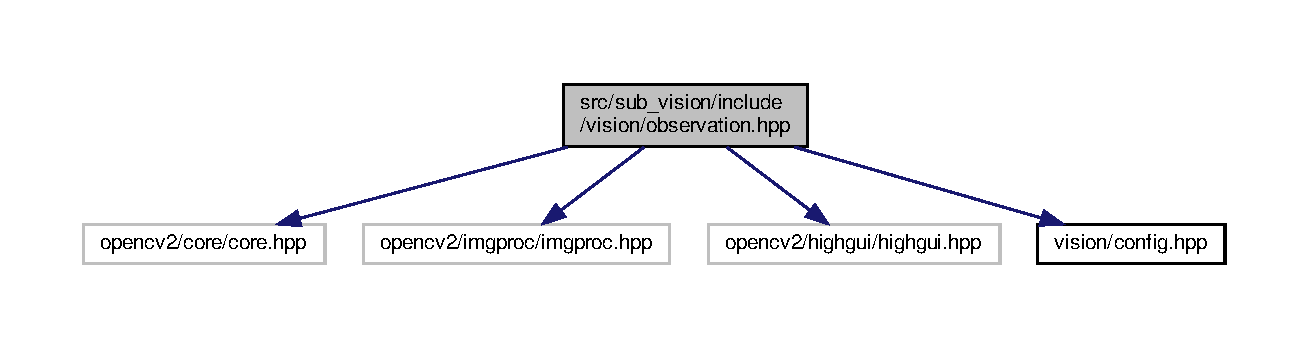
\includegraphics[width=350pt]{observation_8hpp__incl}
\end{center}
\end{figure}
This graph shows which files directly or indirectly include this file\+:
\nopagebreak
\begin{figure}[H]
\begin{center}
\leavevmode
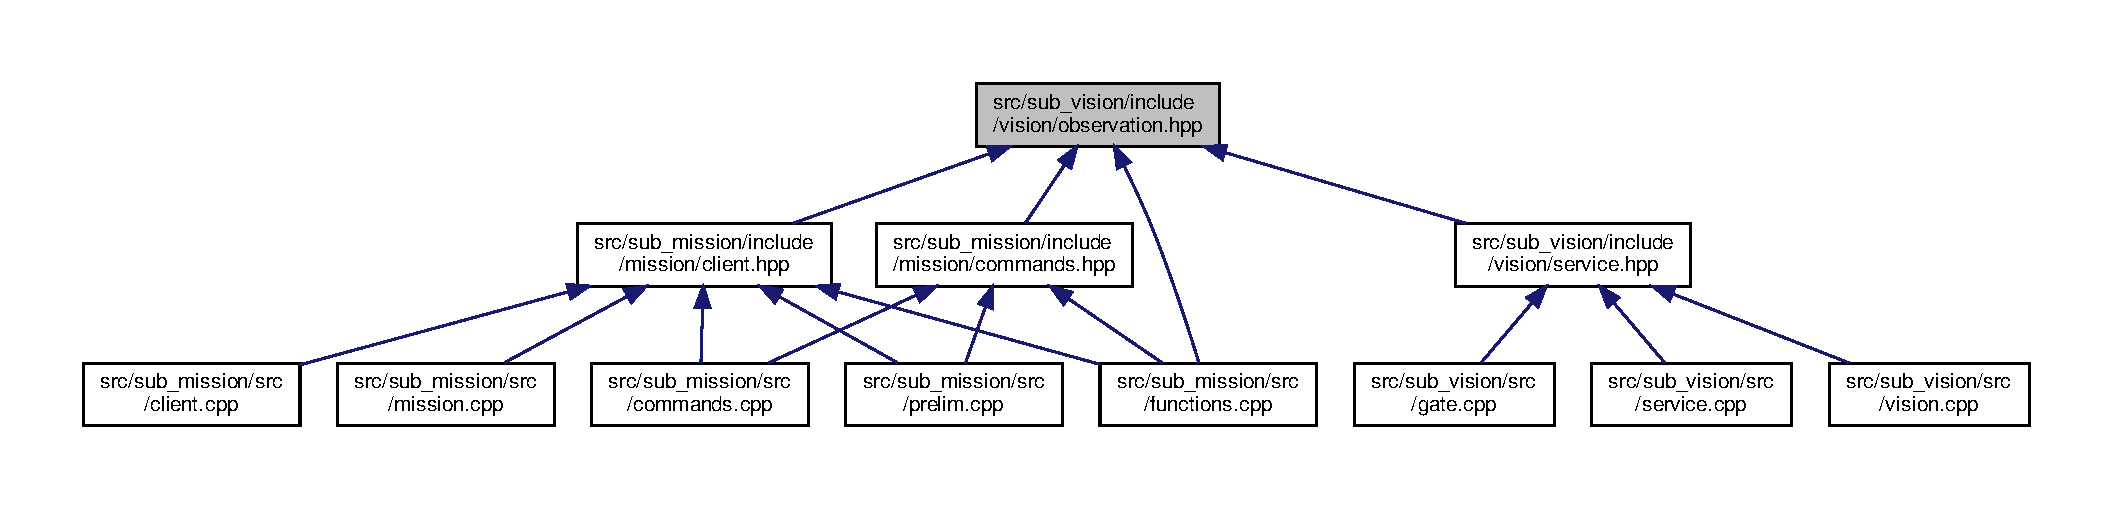
\includegraphics[width=350pt]{observation_8hpp__dep__incl}
\end{center}
\end{figure}
\subsection*{Data Structures}
\begin{DoxyCompactItemize}
\item 
struct \hyperlink{structObservation}{Observation}
\end{DoxyCompactItemize}


\subsection{Detailed Description}
\hyperlink{structObservation}{Observation} struct definition that represents the results from an object detection function. 

\begin{DoxyAuthor}{Author}
David Zhang 
\end{DoxyAuthor}

\hypertarget{tensor_8hpp}{}\section{src/sub\+\_\+vision/include/vision/tensor.hpp File Reference}
\label{tensor_8hpp}\index{src/sub\+\_\+vision/include/vision/tensor.\+hpp@{src/sub\+\_\+vision/include/vision/tensor.\+hpp}}


TF Object Detection A\+PI C++ wrapper for tensors.  


{\ttfamily \#include $<$tensorflow/c/c\+\_\+api.\+h$>$}\newline
{\ttfamily \#include $<$vector$>$}\newline
{\ttfamily \#include $<$string$>$}\newline
{\ttfamily \#include $<$algorithm$>$}\newline
{\ttfamily \#include $<$numeric$>$}\newline
{\ttfamily \#include $<$cstring$>$}\newline
{\ttfamily \#include \char`\"{}vision/model.\+hpp\char`\"{}}\newline
Include dependency graph for tensor.\+hpp\+:\nopagebreak
\begin{figure}[H]
\begin{center}
\leavevmode
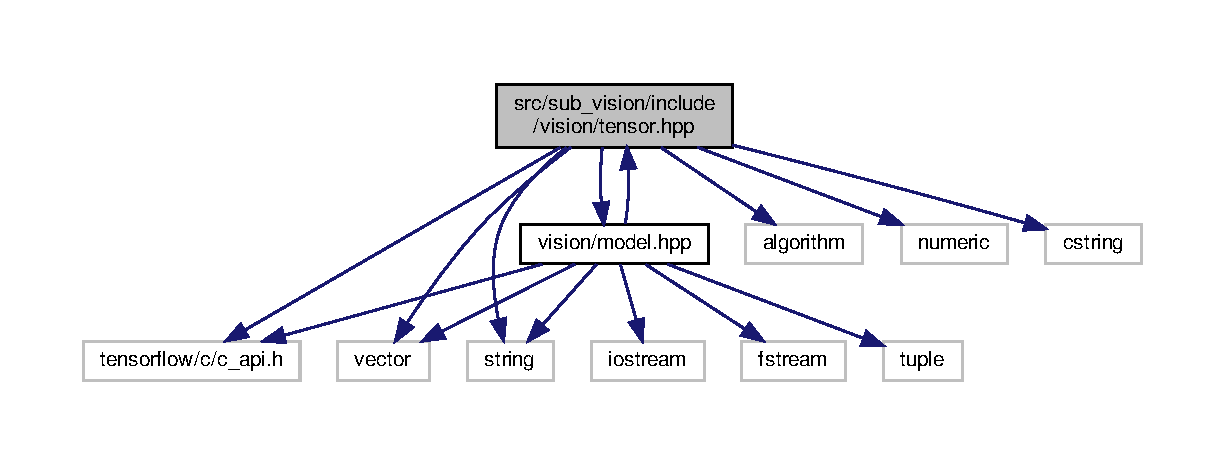
\includegraphics[width=350pt]{tensor_8hpp__incl}
\end{center}
\end{figure}
This graph shows which files directly or indirectly include this file\+:\nopagebreak
\begin{figure}[H]
\begin{center}
\leavevmode
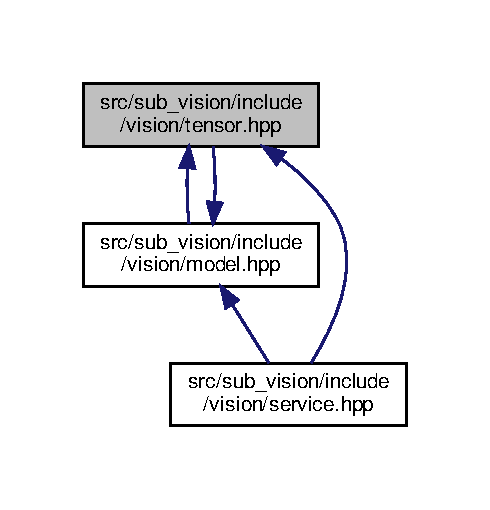
\includegraphics[width=350pt]{tensor_8hpp__dep__incl}
\end{center}
\end{figure}
\subsection*{Data Structures}
\begin{DoxyCompactItemize}
\item 
class \hyperlink{classTensor}{Tensor}
\end{DoxyCompactItemize}


\subsection{Detailed Description}
TF Object Detection A\+PI C++ wrapper for tensors. 

\begin{DoxyAuthor}{Author}
Sergio Izquierdo 
\end{DoxyAuthor}

%--- End generated contents ---

% Index
\backmatter
\newpage
\phantomsection
\clearemptydoublepage
\addcontentsline{toc}{chapter}{Index}
\printindex

\end{document}
